\documentclass[a4paper,11pt,english]{article} 

\usepackage[left=1in,right=1in,top=1in,bottom=1in]{geometry}
\usepackage[utf8]{inputenc} 
\usepackage[T1]{fontenc} 
\usepackage[english]{babel}
\usepackage{amsmath,amsthm,amsfonts,amssymb,amstext} 
\usepackage{textcomp}
\usepackage{upgreek} 
\usepackage[final]{graphicx}      
%\usepackage{epstopdf}
%\usepackage{float} 
\usepackage[font=footnotesize]{caption} 
\usepackage[usenames,dvipsnames]{xcolor} 
%\usepackage{pdfpages} 
%\usepackage{siunitx}
%\captionsetup[figure]{name=Fig.} 
%\captionsetup[table]{name=Tab.} 
\usepackage[bookmarks=true,bookmarksnumbered=true]{hyperref}
%\usepackage[round]{natbib}
%\usepackage{smartdiagram}

\parindent 0cm 
\addtolength{\textheight}{0cm}
\addtolength{\voffset}{0cm} 
\setlength{\parskip}{0.6\baselineskip}

\begin{document}

\title{\textbf{The GALAH survey} \\ Update on spectroscopic analysis pipeline after \textit{Gaia} DR2}
\author{WG4 - Sven Buder, contributions by A. M. Amarsi, J. Lin, K. Lind, T. Nordlander}

\maketitle

\section{Important changes after GALAH and \textit{Gaia} DR2}

\subsection{Documentation, spectroscopic synthesis pipeline, and code for data processing available for members}

The spectroscopic synthesis pipeline is now open for all GALAH members to use via

\url{https://galah-survey.org/wiki/galah-spectrum-synthesis-pipeline}

If you are not a member of WG4, we ask you to please do not share the credentials with non-members or commit files to the SVN!

Documents and code for analyses and data processing have been uploaded on a private (hidden) repository. If you want to access to these documents, please email Sven to be added as a collaborator (you need a github account for this!).

\subsection{Updates regarding Spectroscopy Made Ease (SME)}

\begin{itemize}
\item Pipeline finally and successfully converted to the recent SME version 536 (if interested, ask WG4 regarding the major changes). Thanks to Thomas Nordlander!
\item Improved continuum selection and normalisation with SME. Thanks to Karin Lind!
\item Non-LTE now also for H (in addition to Li, O, Na, Mg, Al, Si, and Fe). Thanks to Anish Amarsi!
\end{itemize}

\subsection{Updates regarding use of \textit{Gaia} DR2 and asterseismic data}

\begin{figure}[!ht]
\centering
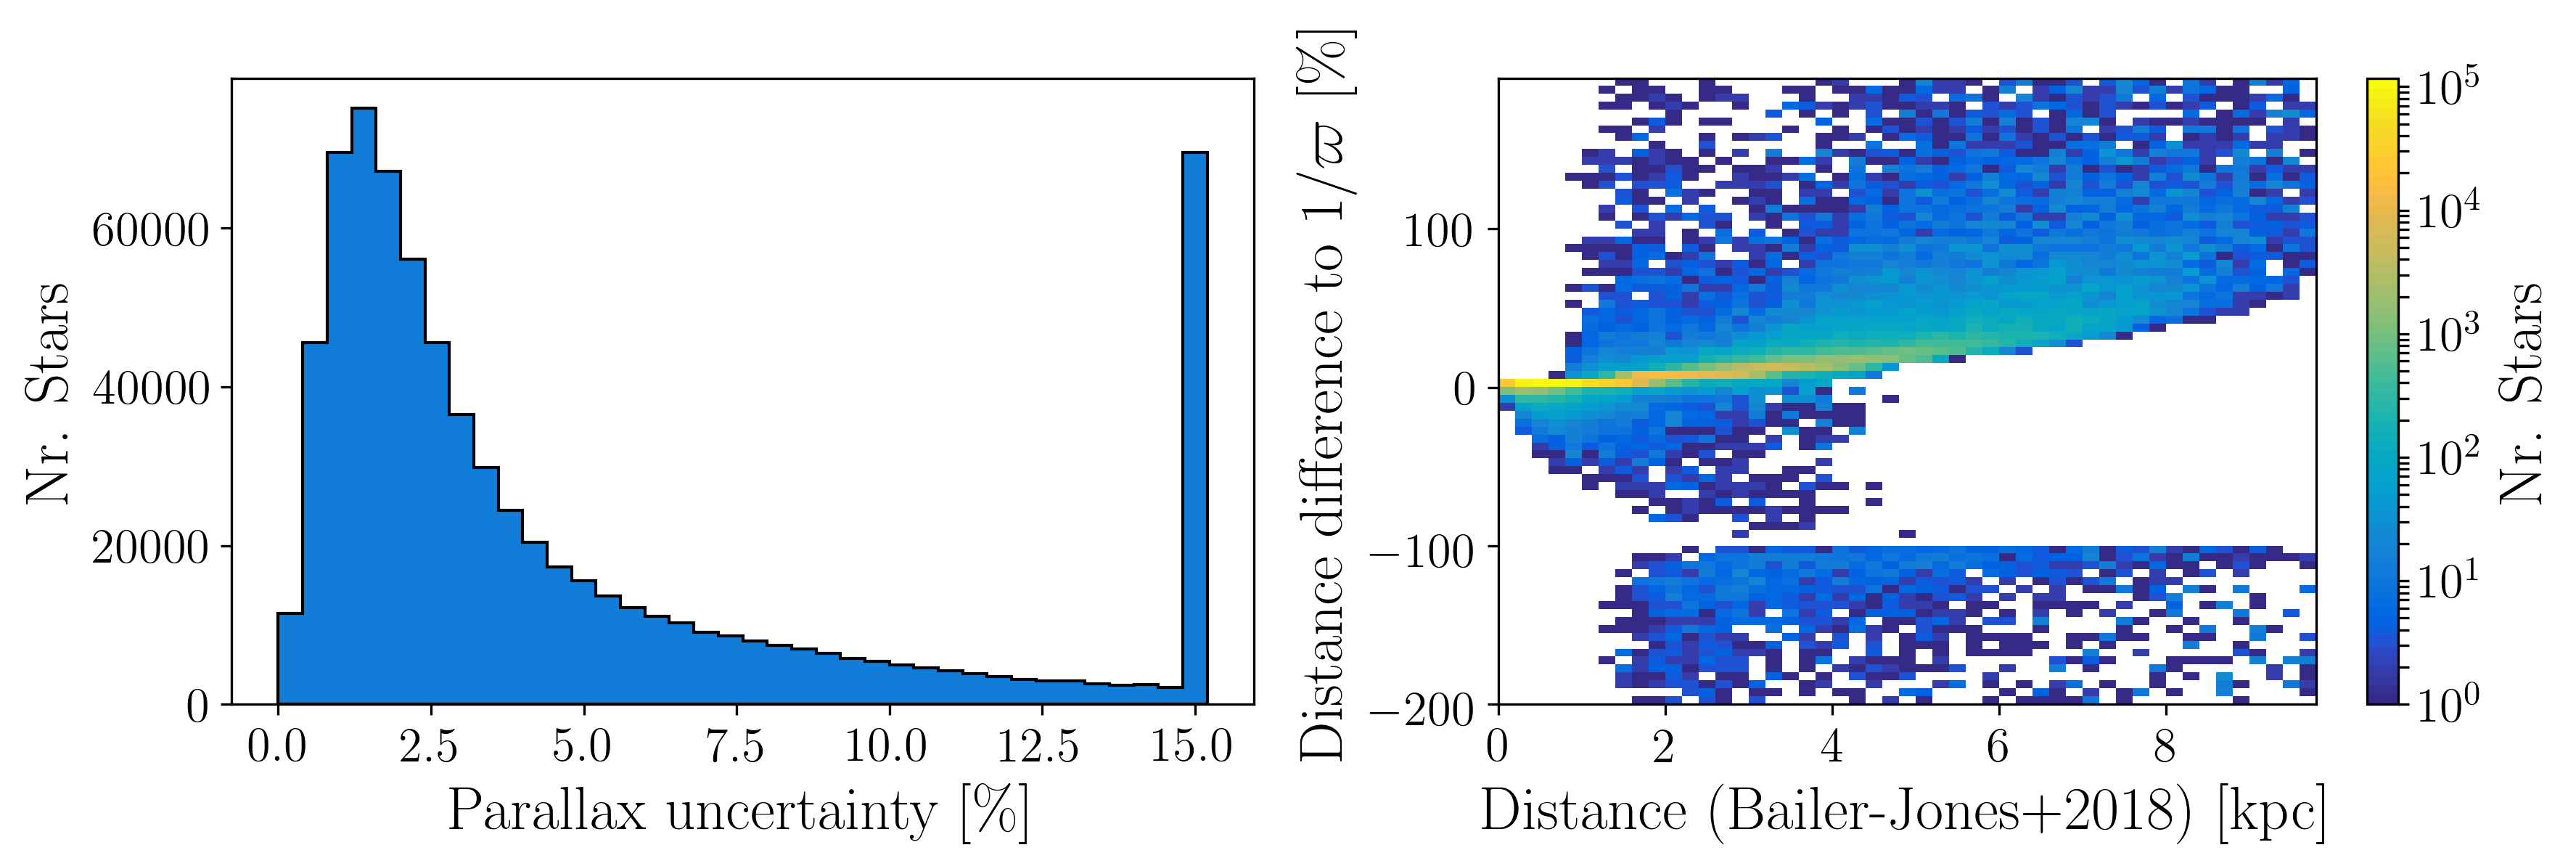
\includegraphics[width=\textwidth]{../../input/figures/parallax_uncertainties.png}
\caption{Overview of parallaxes/distances of the stars observed by GALAH.}
\label{fig:parallax_overview}
\end{figure}

\begin{itemize}
\item Parallaxes are now available for almost all stars observed by GALAH and a vast majority of them are very good, see \autoref{fig:parallax_overview}. Overall, currently 728651 spectra have matched parallax measurements, 85\% (619333) even with parallax uncertainty $< 10\%$. When dividing the sample into giants ($\textsc{teff\_guess} < 5500\,\mathrm{K}$ and $M_{K_S} < 2\,\mathrm{mag}$), 93 \% (454406/488192) of the observed dwarf spectra have parallax uncertainties below 10 \% and 69 \% (164927/240459) of the observed giant spectra have parallax uncertainties below 10 \%. For the analysis, we use the inferred distance estimates by Bailer-Jones et al. (2018), which is most important for the largest parallax uncertainties (see right panel of \autoref{fig:parallax_overview}).
\item The asteroseismic information provided by Sanjib Sharma and others have been used to run a pipeline version which constrains $\log g$ as a function of $T_\text{eff}$ and $\nu_\text{max}$, which consists of up to 3175 spectra (including bad S/N, bad $\nu_text{max}$ values, and bad reductions).
\item For the interim mass and age estimation, we have switched to the use of Parsec isochrones, which include core helium burning stars (in contrast to Dartmouth isochrones) and alpha-enhancement (in contrast to MIST). Thanks to Jane Lin!
\end{itemize}

\section{Performances}

\begin{figure}[!ht]
\centering
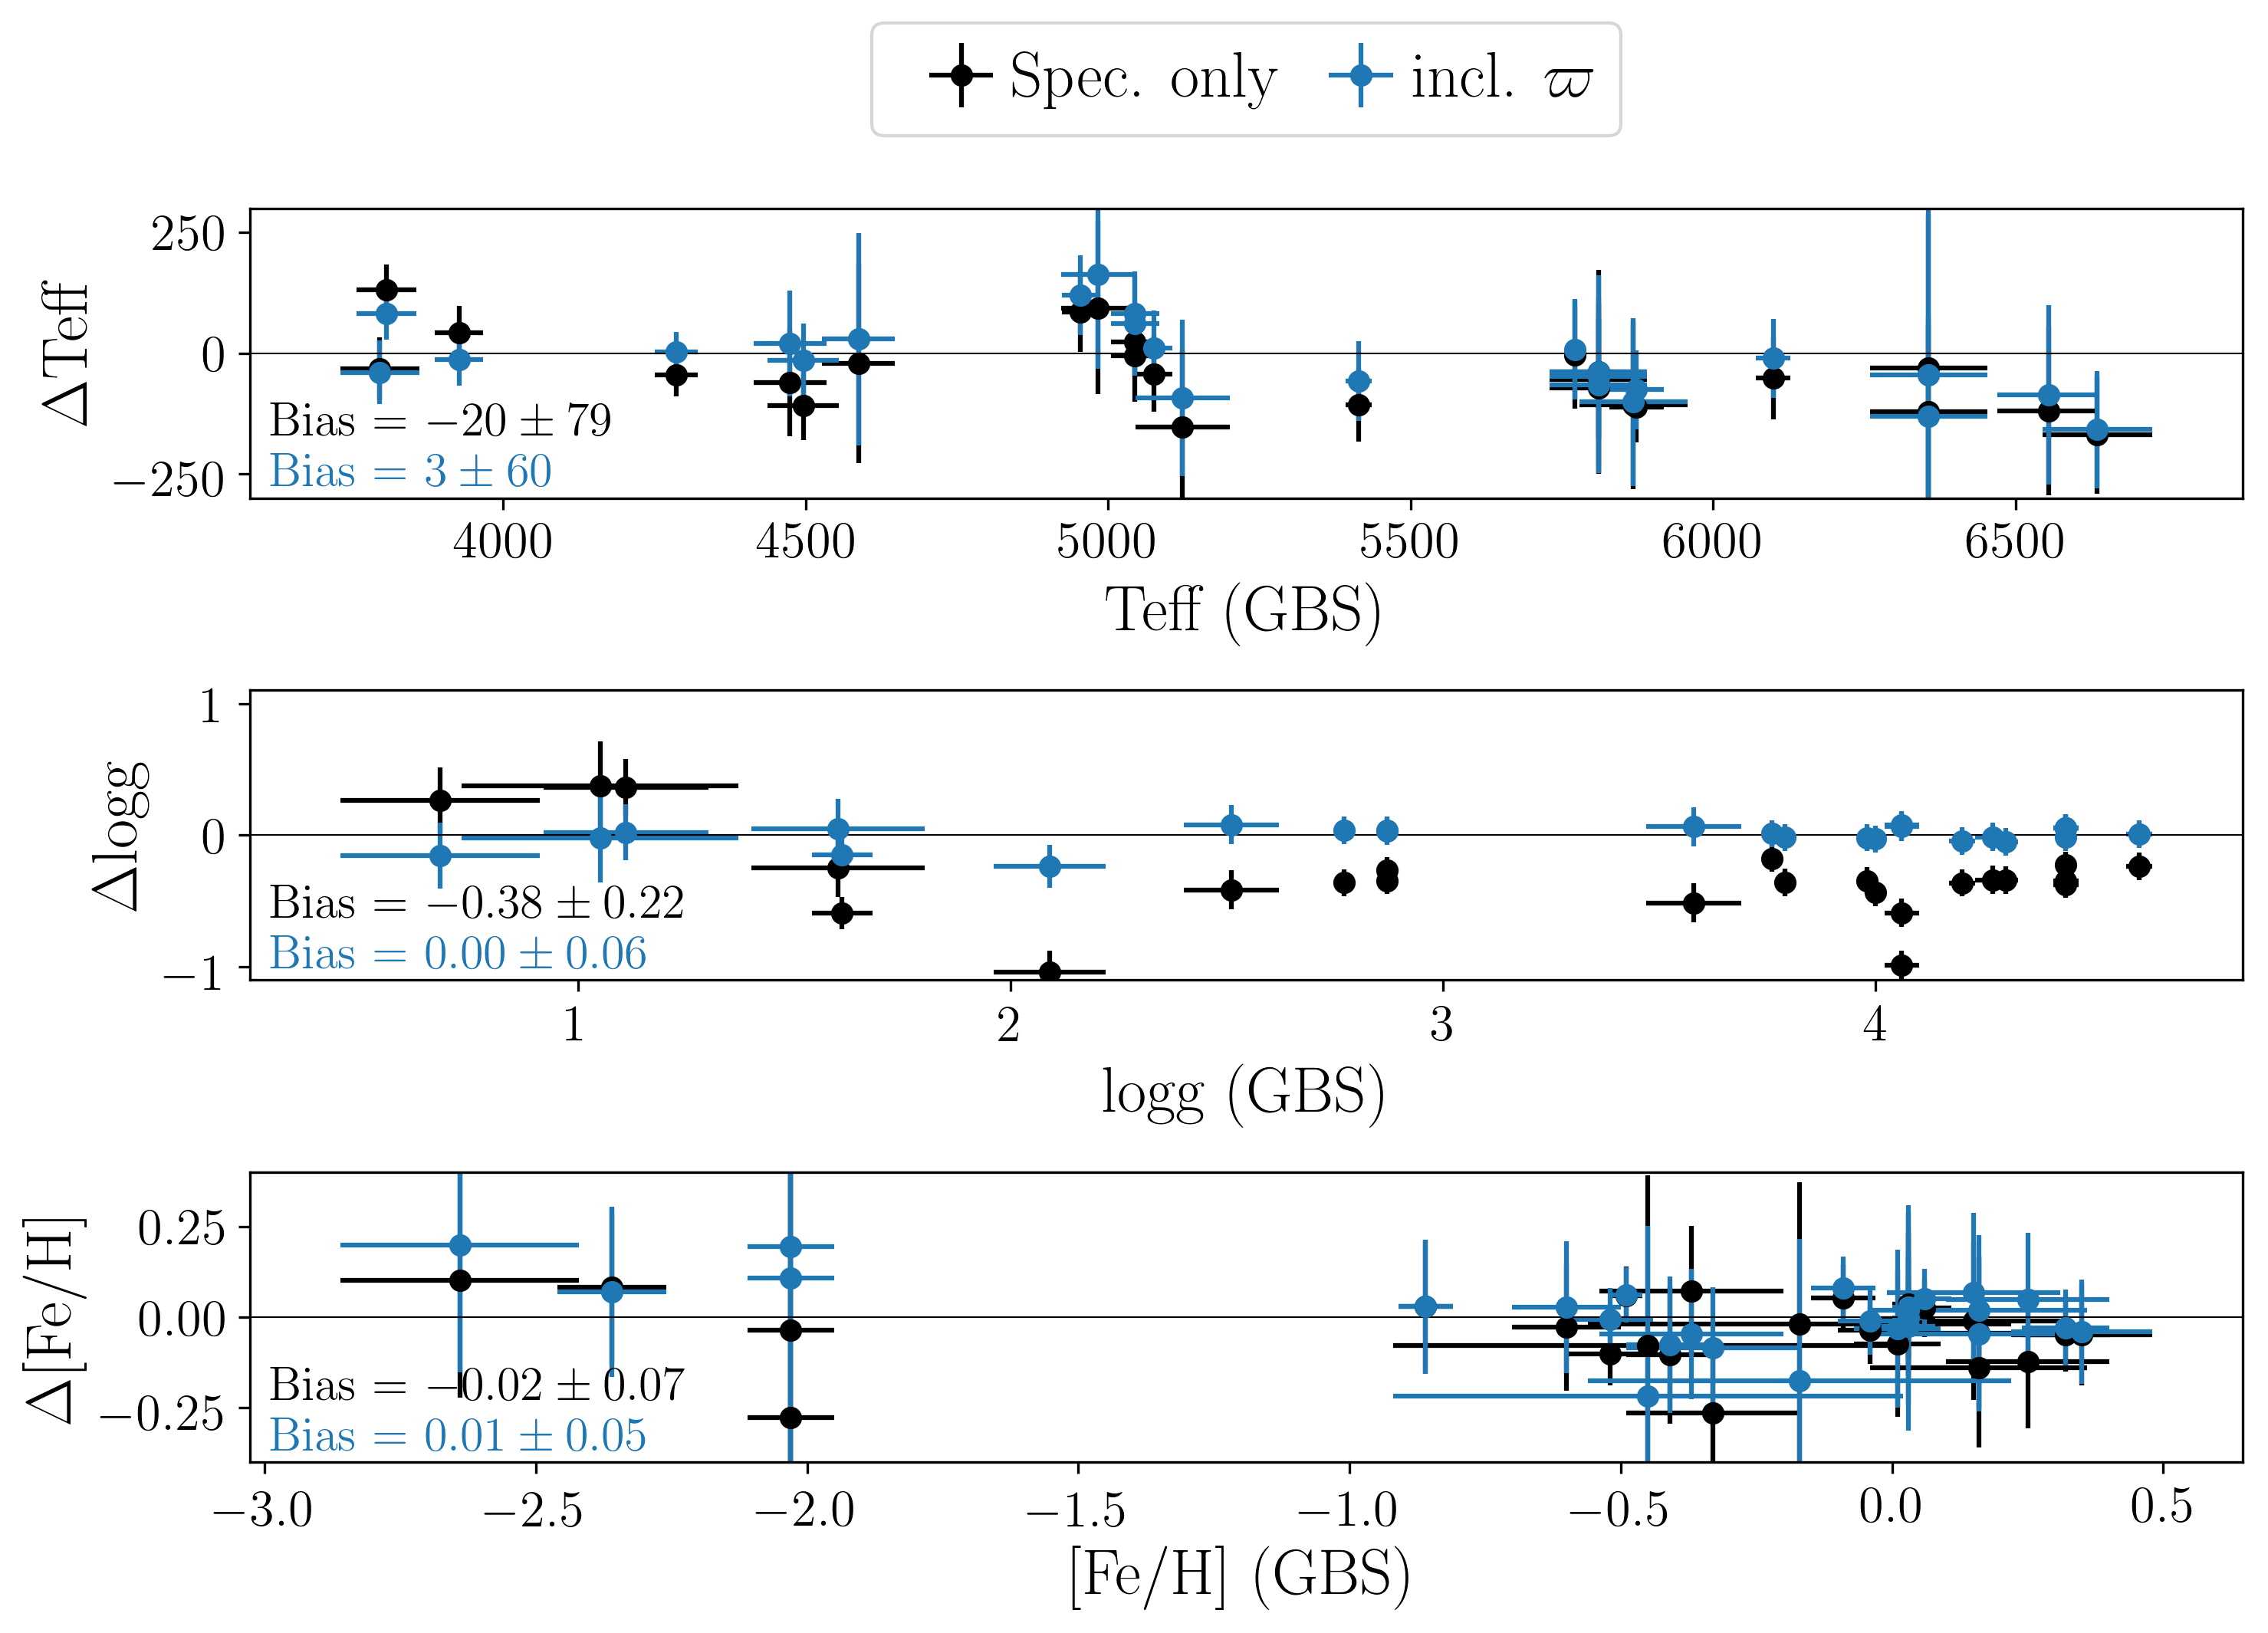
\includegraphics[width=0.9\textwidth]{../../gbs/figures/gbs_performance_free_lbol.png}
\caption{Performance of GALAH synthesis pipeline without (black) and with (blue) bolometric information.}
\label{fig:gbs_performance}
\end{figure}

\subsection{\textit{Gaia} FGK benchmark stars (GBS)}

For the bolometric pipeline, we do not find any significant biases among the GBS regarding $T_\text{eff}$ and $\log g$, but had to correct a bias of $\mathrm{[Fe/H]}  = -0.1$ (underestimated [Fe/H]), see \autoref{fig:gbs_performance}. Underestimated temperatures for the hottest stars are still likely, but more testing is needed as the continuum normalisation has been improved and hydrogen has been implemented in non-LTE now. More importantly, the scatter with respect to the GBS values by Jofré et al. (2018) has decreased significantly for $\log g$ and noticeably for $T_\text{eff}$ and $\mathrm{[Fe/H]}$.

\subsection{Stars with asteroseismic information}

The analyses of the overlap of the stars with asteroseismic parameters and parallaxes, see \autoref{fig:seis_comparison1}, show that the bolometric pipeline (middle panels) performs significantly better than the pipeline without additional non-spectroscopic information (left panels). Especially the Red Clump stars show an outstanding agreement with the pipeline results which also used $\nu_\text{max}$ values.

\begin{figure}[!ht]
\centering
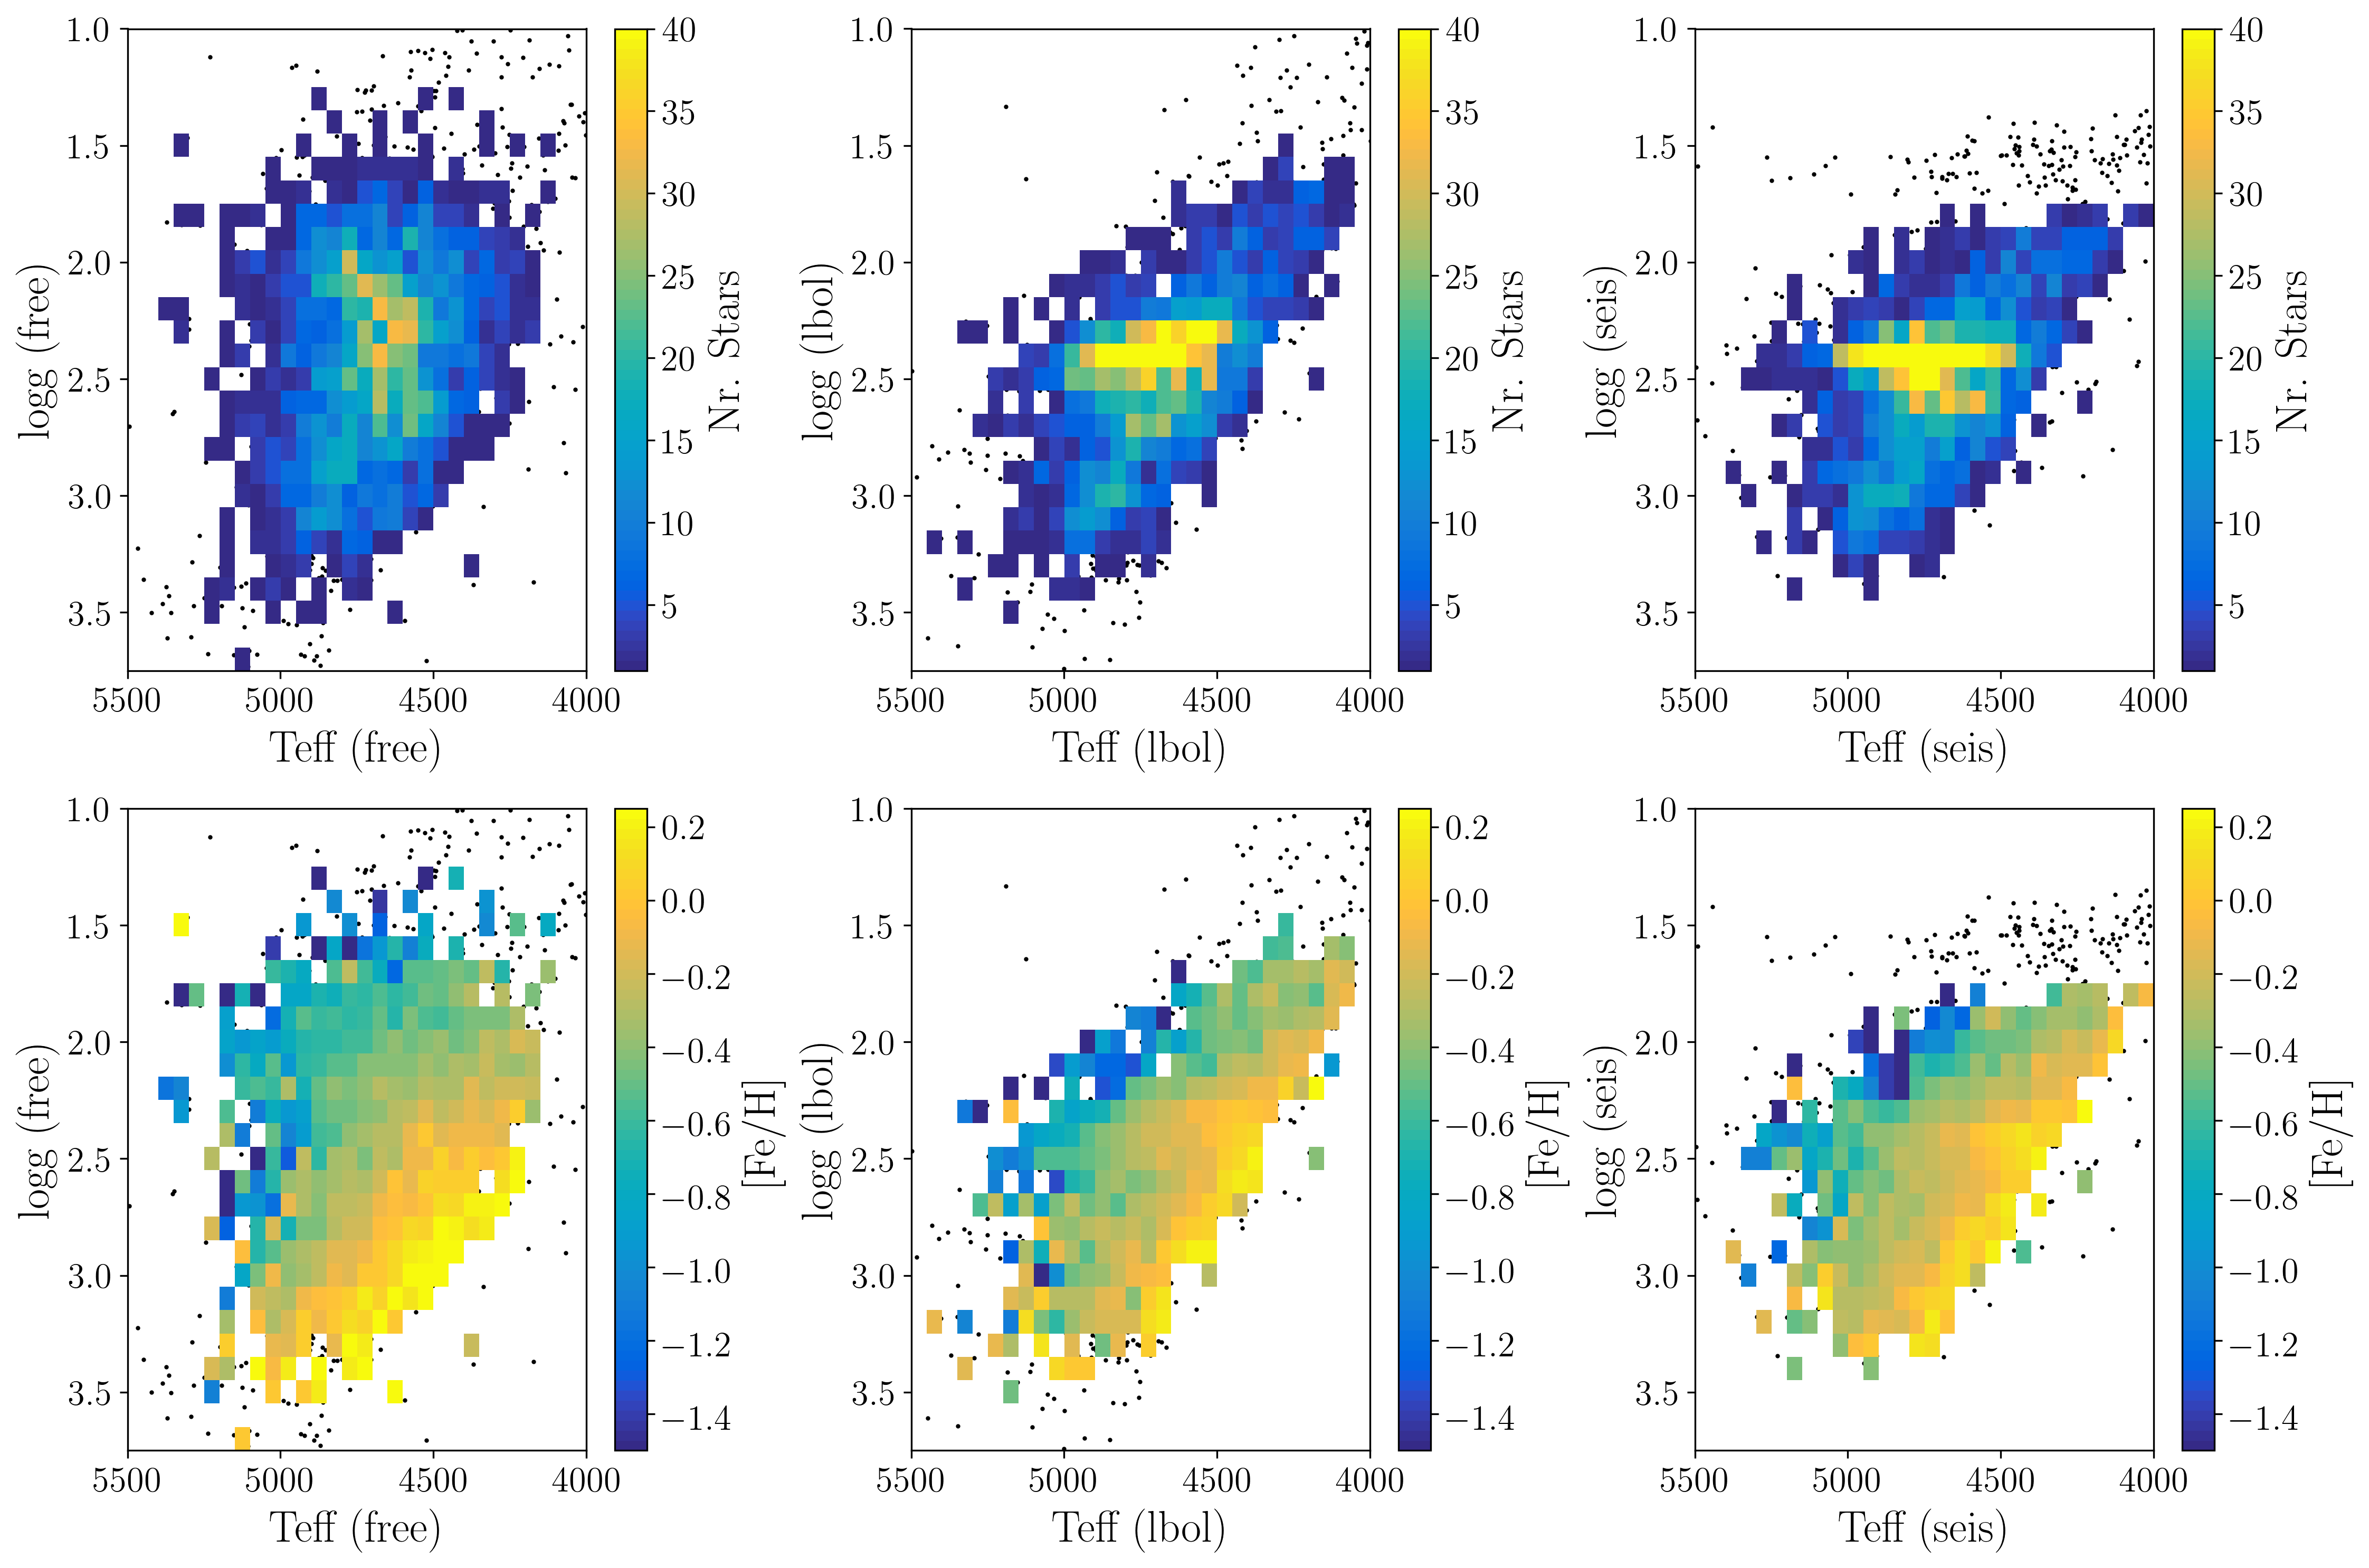
\includegraphics[width=\textwidth]{../../seis/figures/seis_comparison_3setups.png}
\caption{Kiel diagrams showing the performances of the three GALAH synthesis pipelines for the stars with asteroseismic information ($\log g = f(T_\text{eff}, \nu_\text{max})$) and bolometric information ($\log g = f(M, T_\text{eff}, \varpi, BC, K_S, A_{K_S})$), with top plots for density and bottom plots colored by mean [Fe/H]. Left panels show the results without additional non-spectroscopic information, middle panels when using bolometric information and right panels when using asteroseismic information.}
\label{fig:seis_comparison1}
\end{figure}

The scatter in the differences between asteroseismic and bolometric pipeline for logg is mainly driven by the red clump stars, which have to be further investigated, but are significantly better than for GALAH DR2, see the right hand plot in \autoref{fig:seis_comparison2}.

\begin{figure}[!ht]
\centering
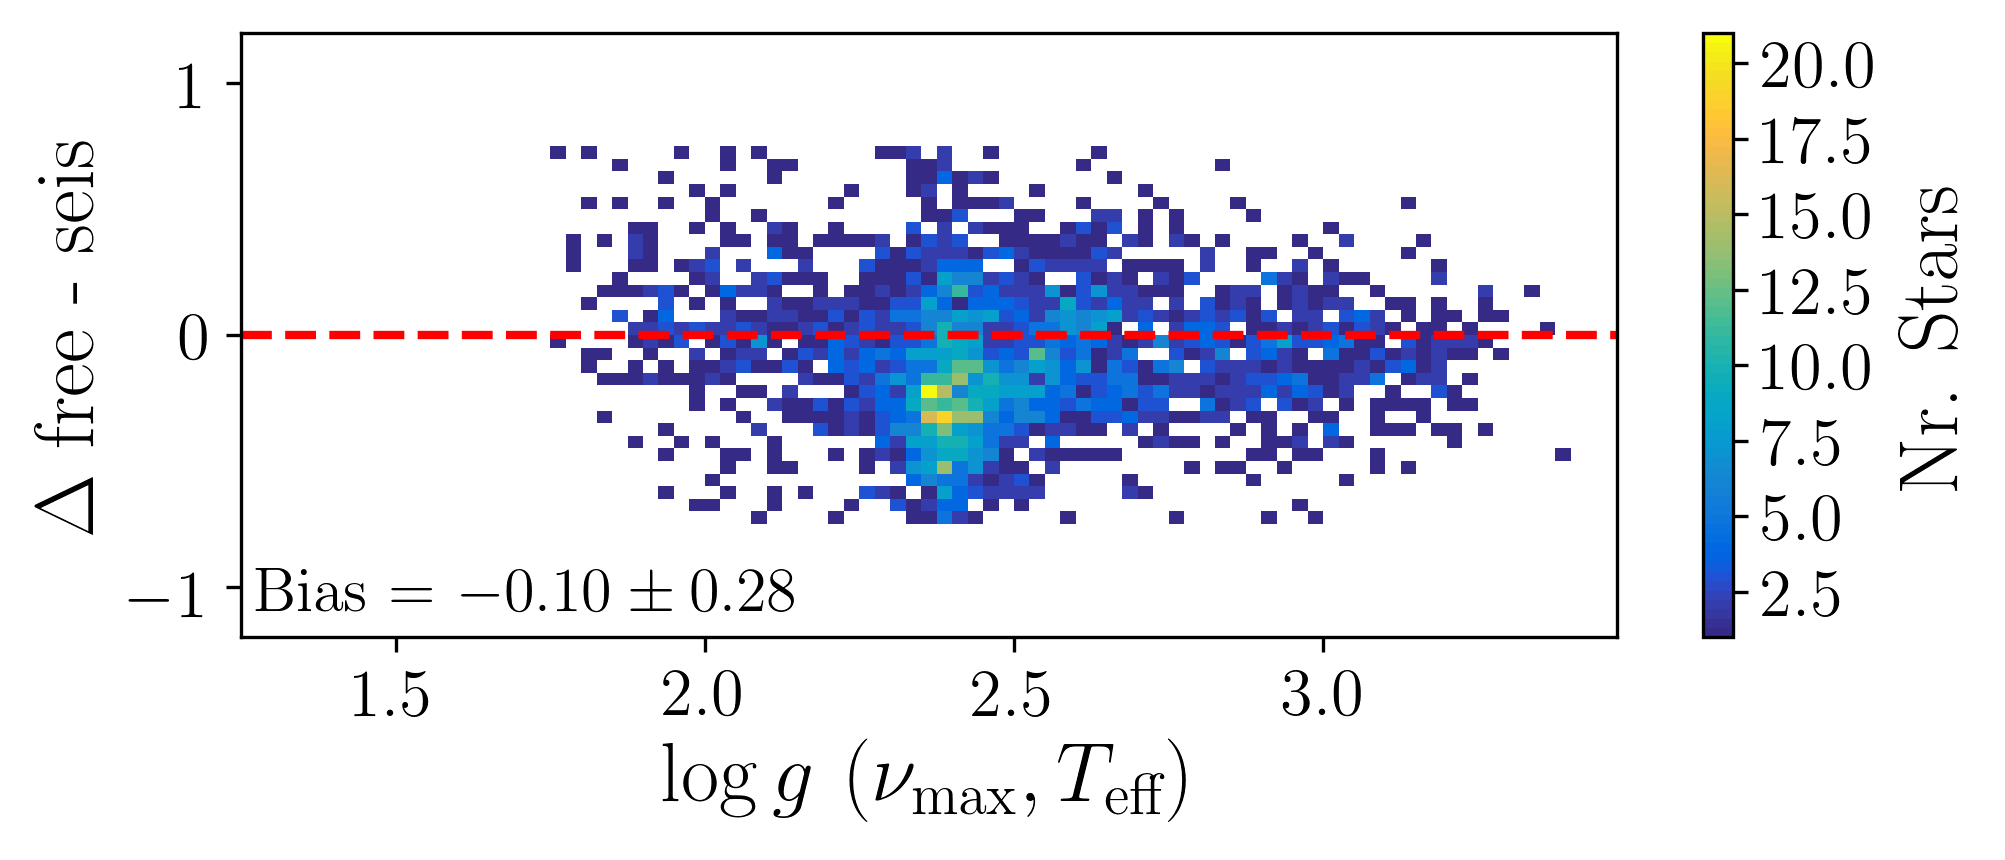
\includegraphics[width=0.49\textwidth]{../../seis/figures/seismic_sample_delta_free.png}
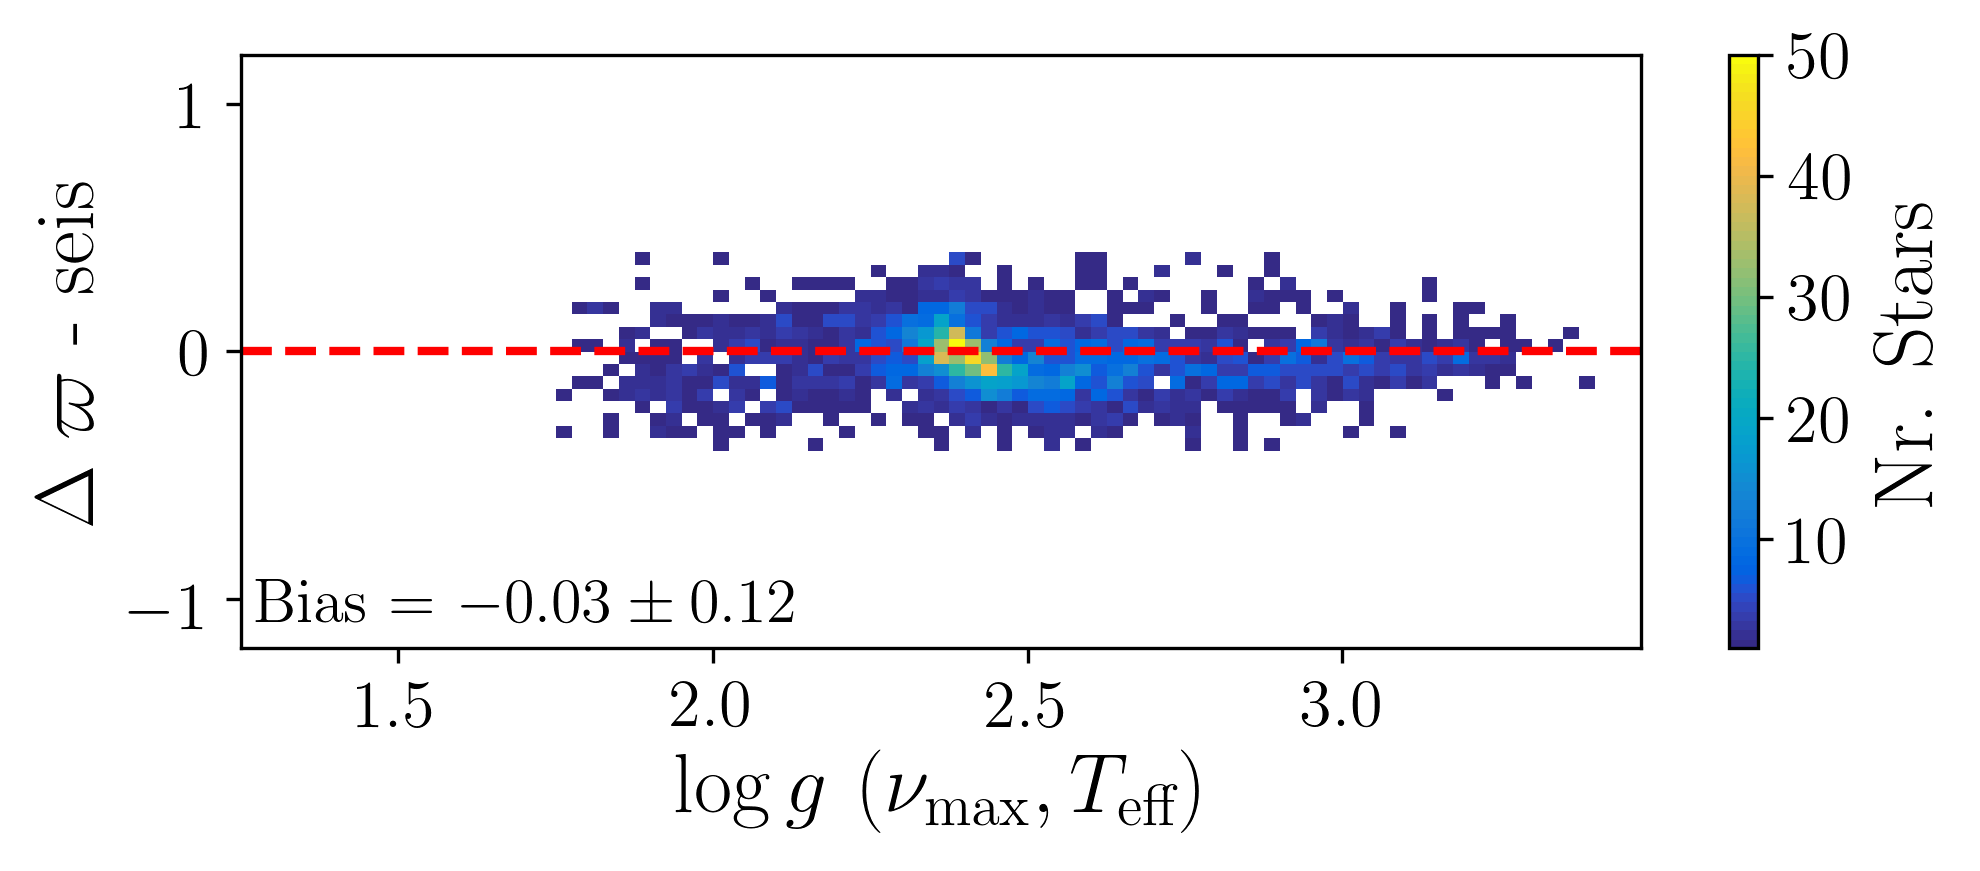
\includegraphics[width=0.49\textwidth]{../../seis/figures/seismic_sample_delta_lbol.png}
\caption{Difference of $\log g$ for stars with asteroseismic sample. Left: $\log g$ (free - seis). Right: $\log g$ (lbol - seis)}
\label{fig:seis_comparison2}
\end{figure}

\begin{figure}[!ht]
\centering
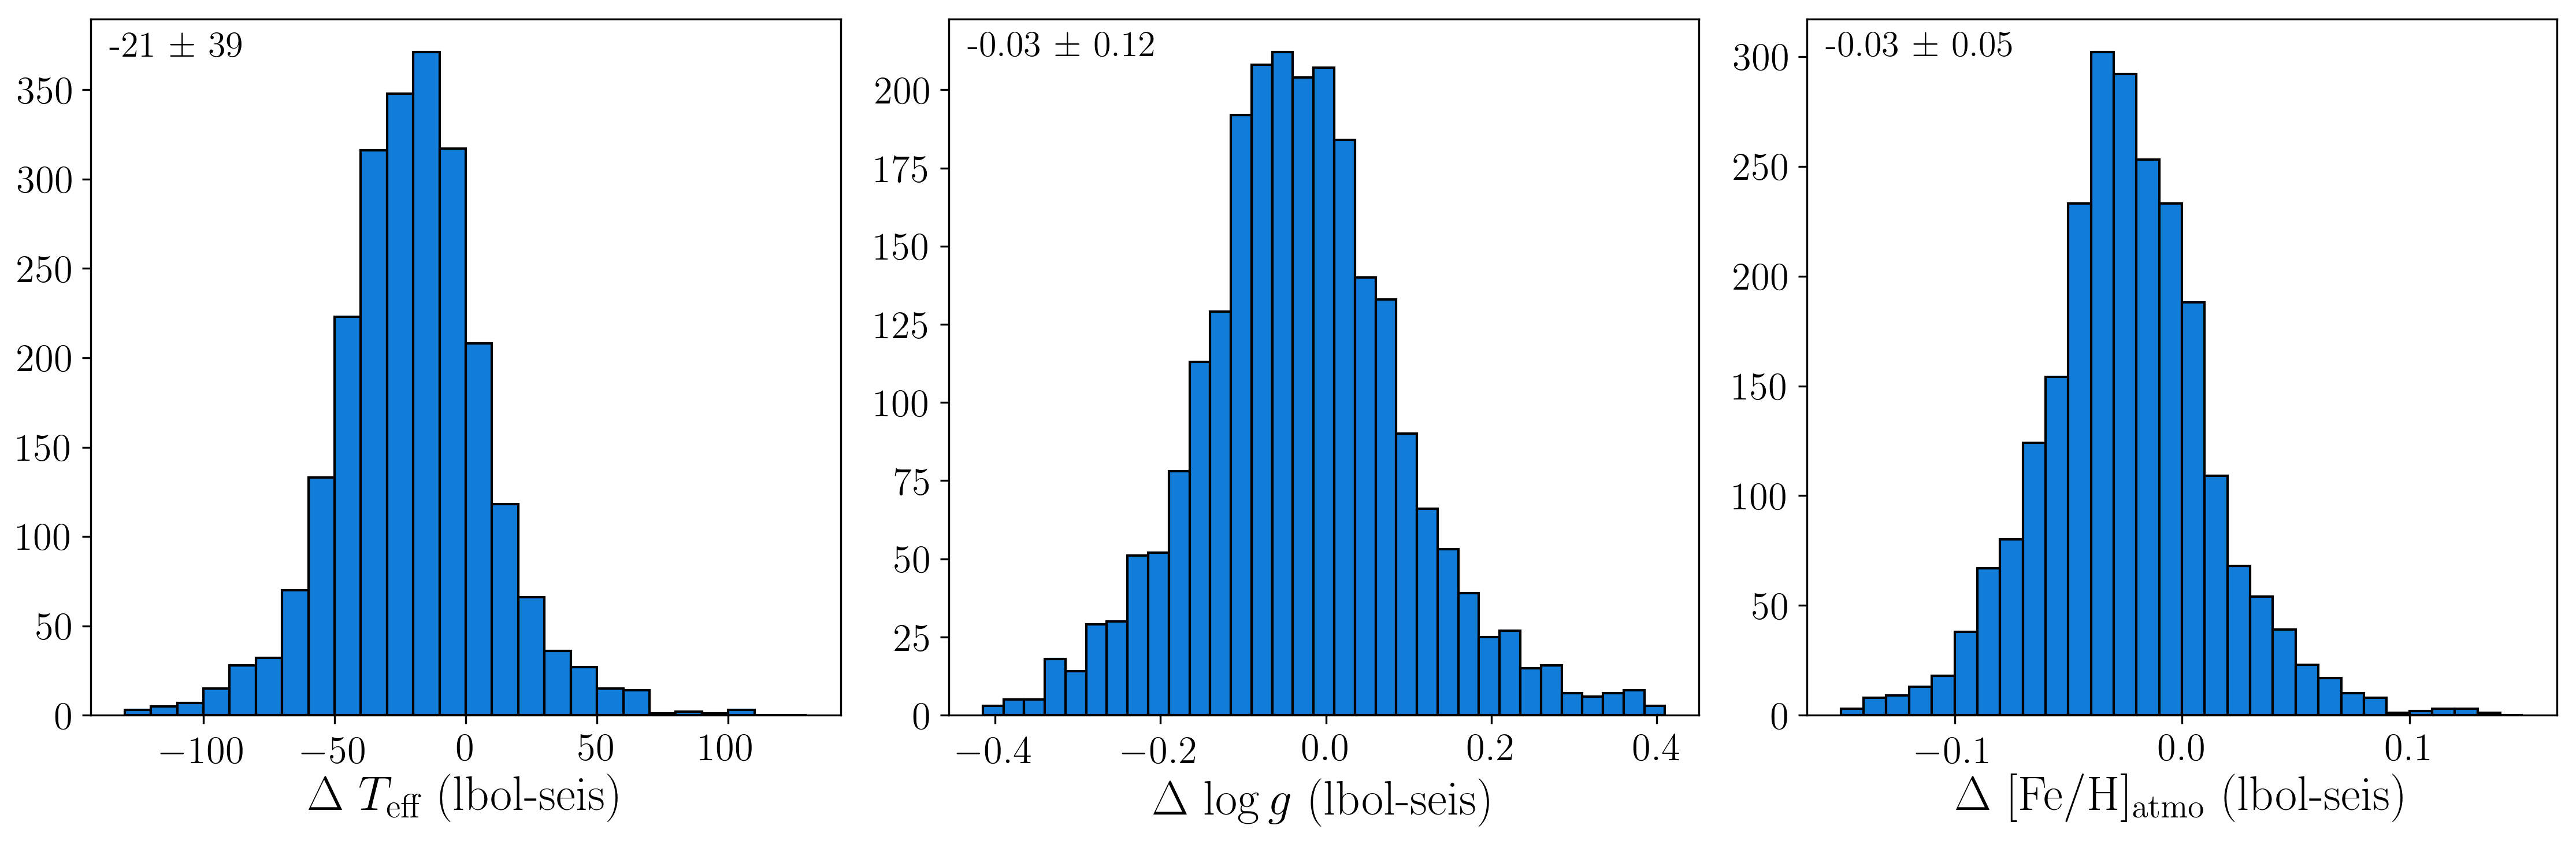
\includegraphics[width=\textwidth]{../../seis/figures/seis_setup_difference_lbol.png}
\caption{Differences (lbol - seis setups) of stellar parameters (left $T_\text{eff}$, middle $\log g$, right [Fe/H] for the stars with asteroseismic information.}
\label{fig:seis_comparison3}
\end{figure}

The biases between asteroseismic and bolometric pipelines for the stellar parameters are not significant but show a trend of lower Teff (-21K), lower logg (-0.03dex), and lower [Fe/H] (-0.03dex) than the values from the pipeline using asteroseismic values/relations for logg.

\subsection{Stars in clusters}

Based on the cluster membership analysis by Janez Kos, we have calculated the stellar parameters for all open and globular cluster members, for which an overview in forms of CMD, Kiel diagram, and distribution of [Fe/H] and interim ages (only maximum likelihood isochrone interpolation) can be found in \autoref{fig:cluster_overview}.

\begin{figure}[!ht]
\centering
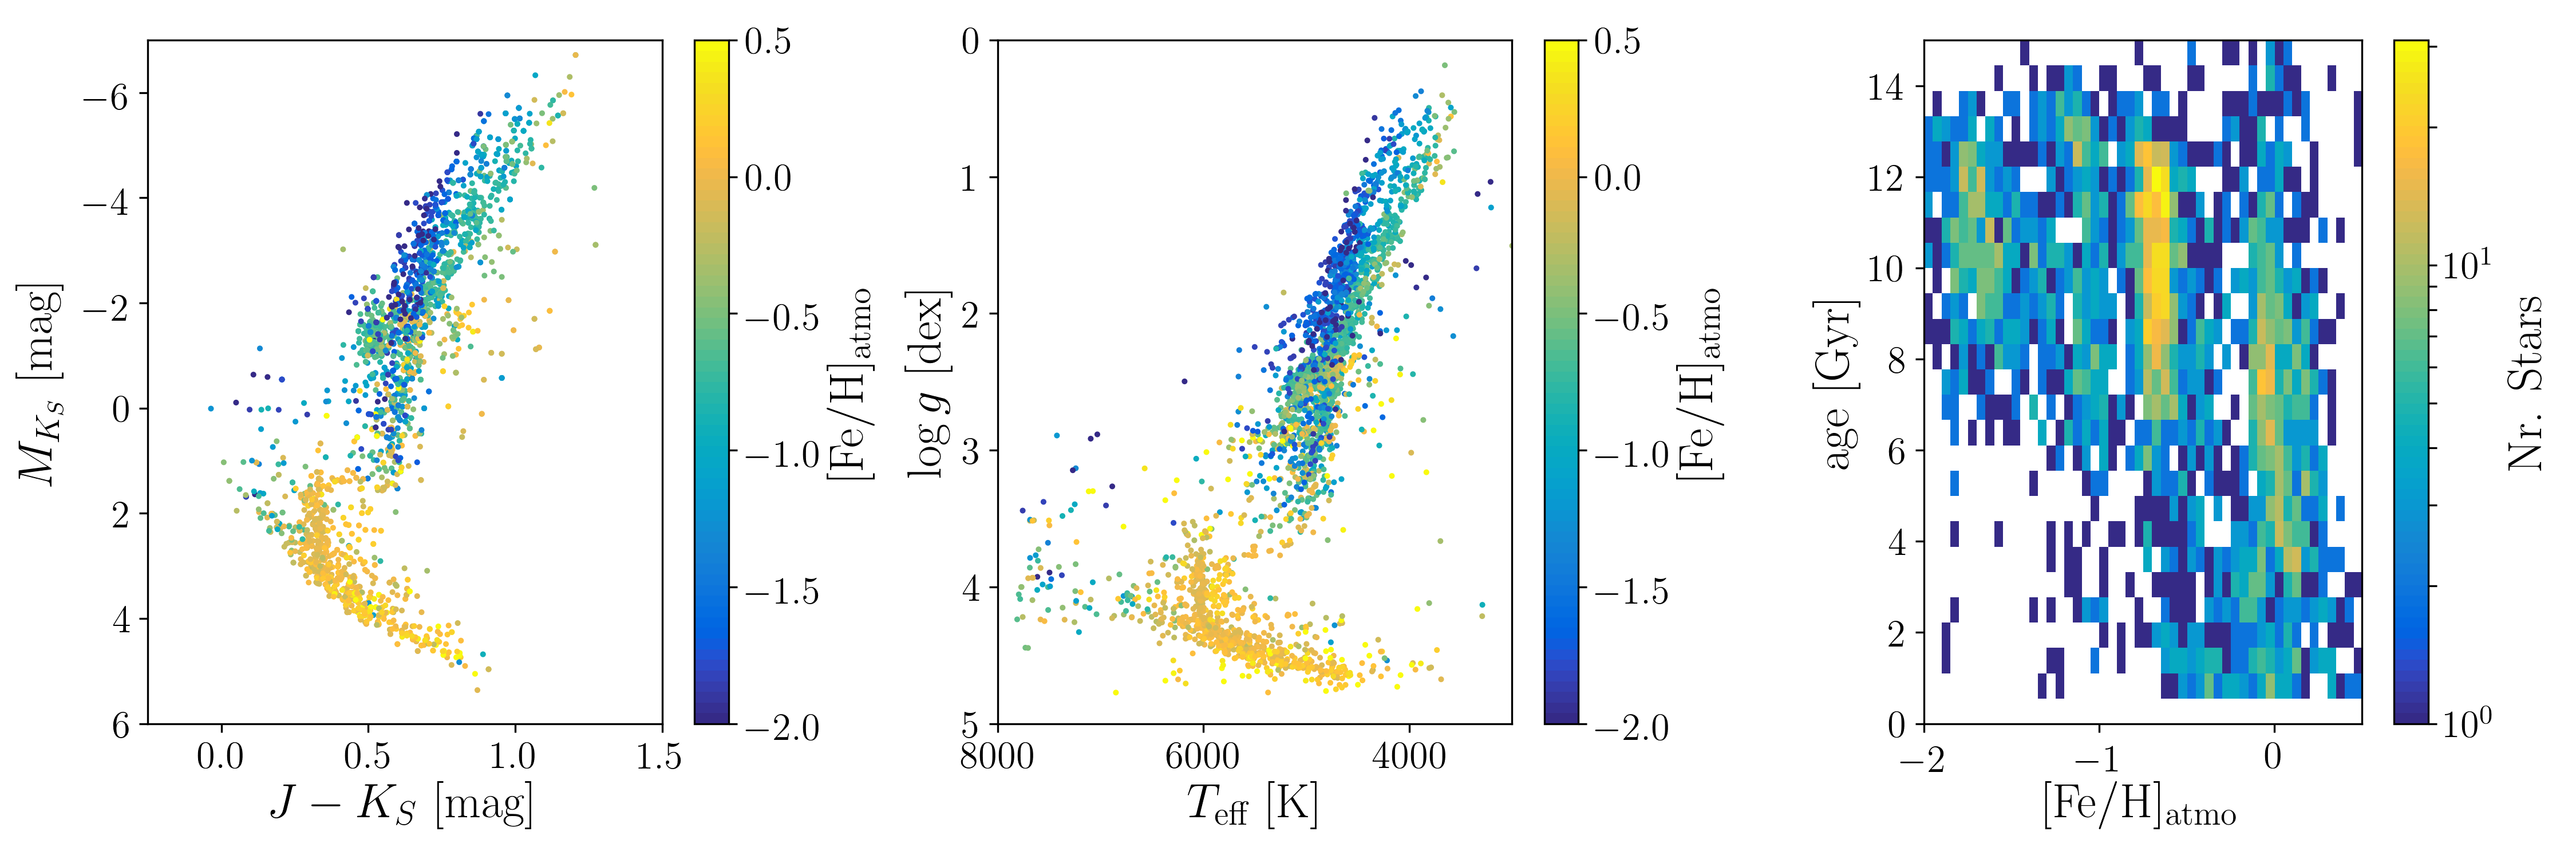
\includegraphics[width=\textwidth]{../../clusters/figures/CMD_Kiel_FehAge.png}
\caption{Overview of cluster stars observed by GALAH.}
\label{fig:cluster_overview}
\end{figure}

\subsection{Performance for star of the GALAH DR2 training set}

We have reanalysed the training set used for GALAH DR2 (see Fig. 9 in Buder et al., 2018), with the available information from \textit{Gaia} DR2, see \autoref{fig:dr2_rerun_kiel}. The stellar parameters have significantly improved in accuracy and precision. The scatter of parameters of the red clump stars has decreased. The constraints on $\log g$ have solved degeneracies for the giant stars, leading to a narrow RGB even for the lowest $\log g$ also leading to more reliable $T_\text{eff}$ and $\mathrm{[Fe/H]}$. Improvements on the pipeline have also lead to a more narrow main sequence.

\begin{figure}[!ht]
\centering
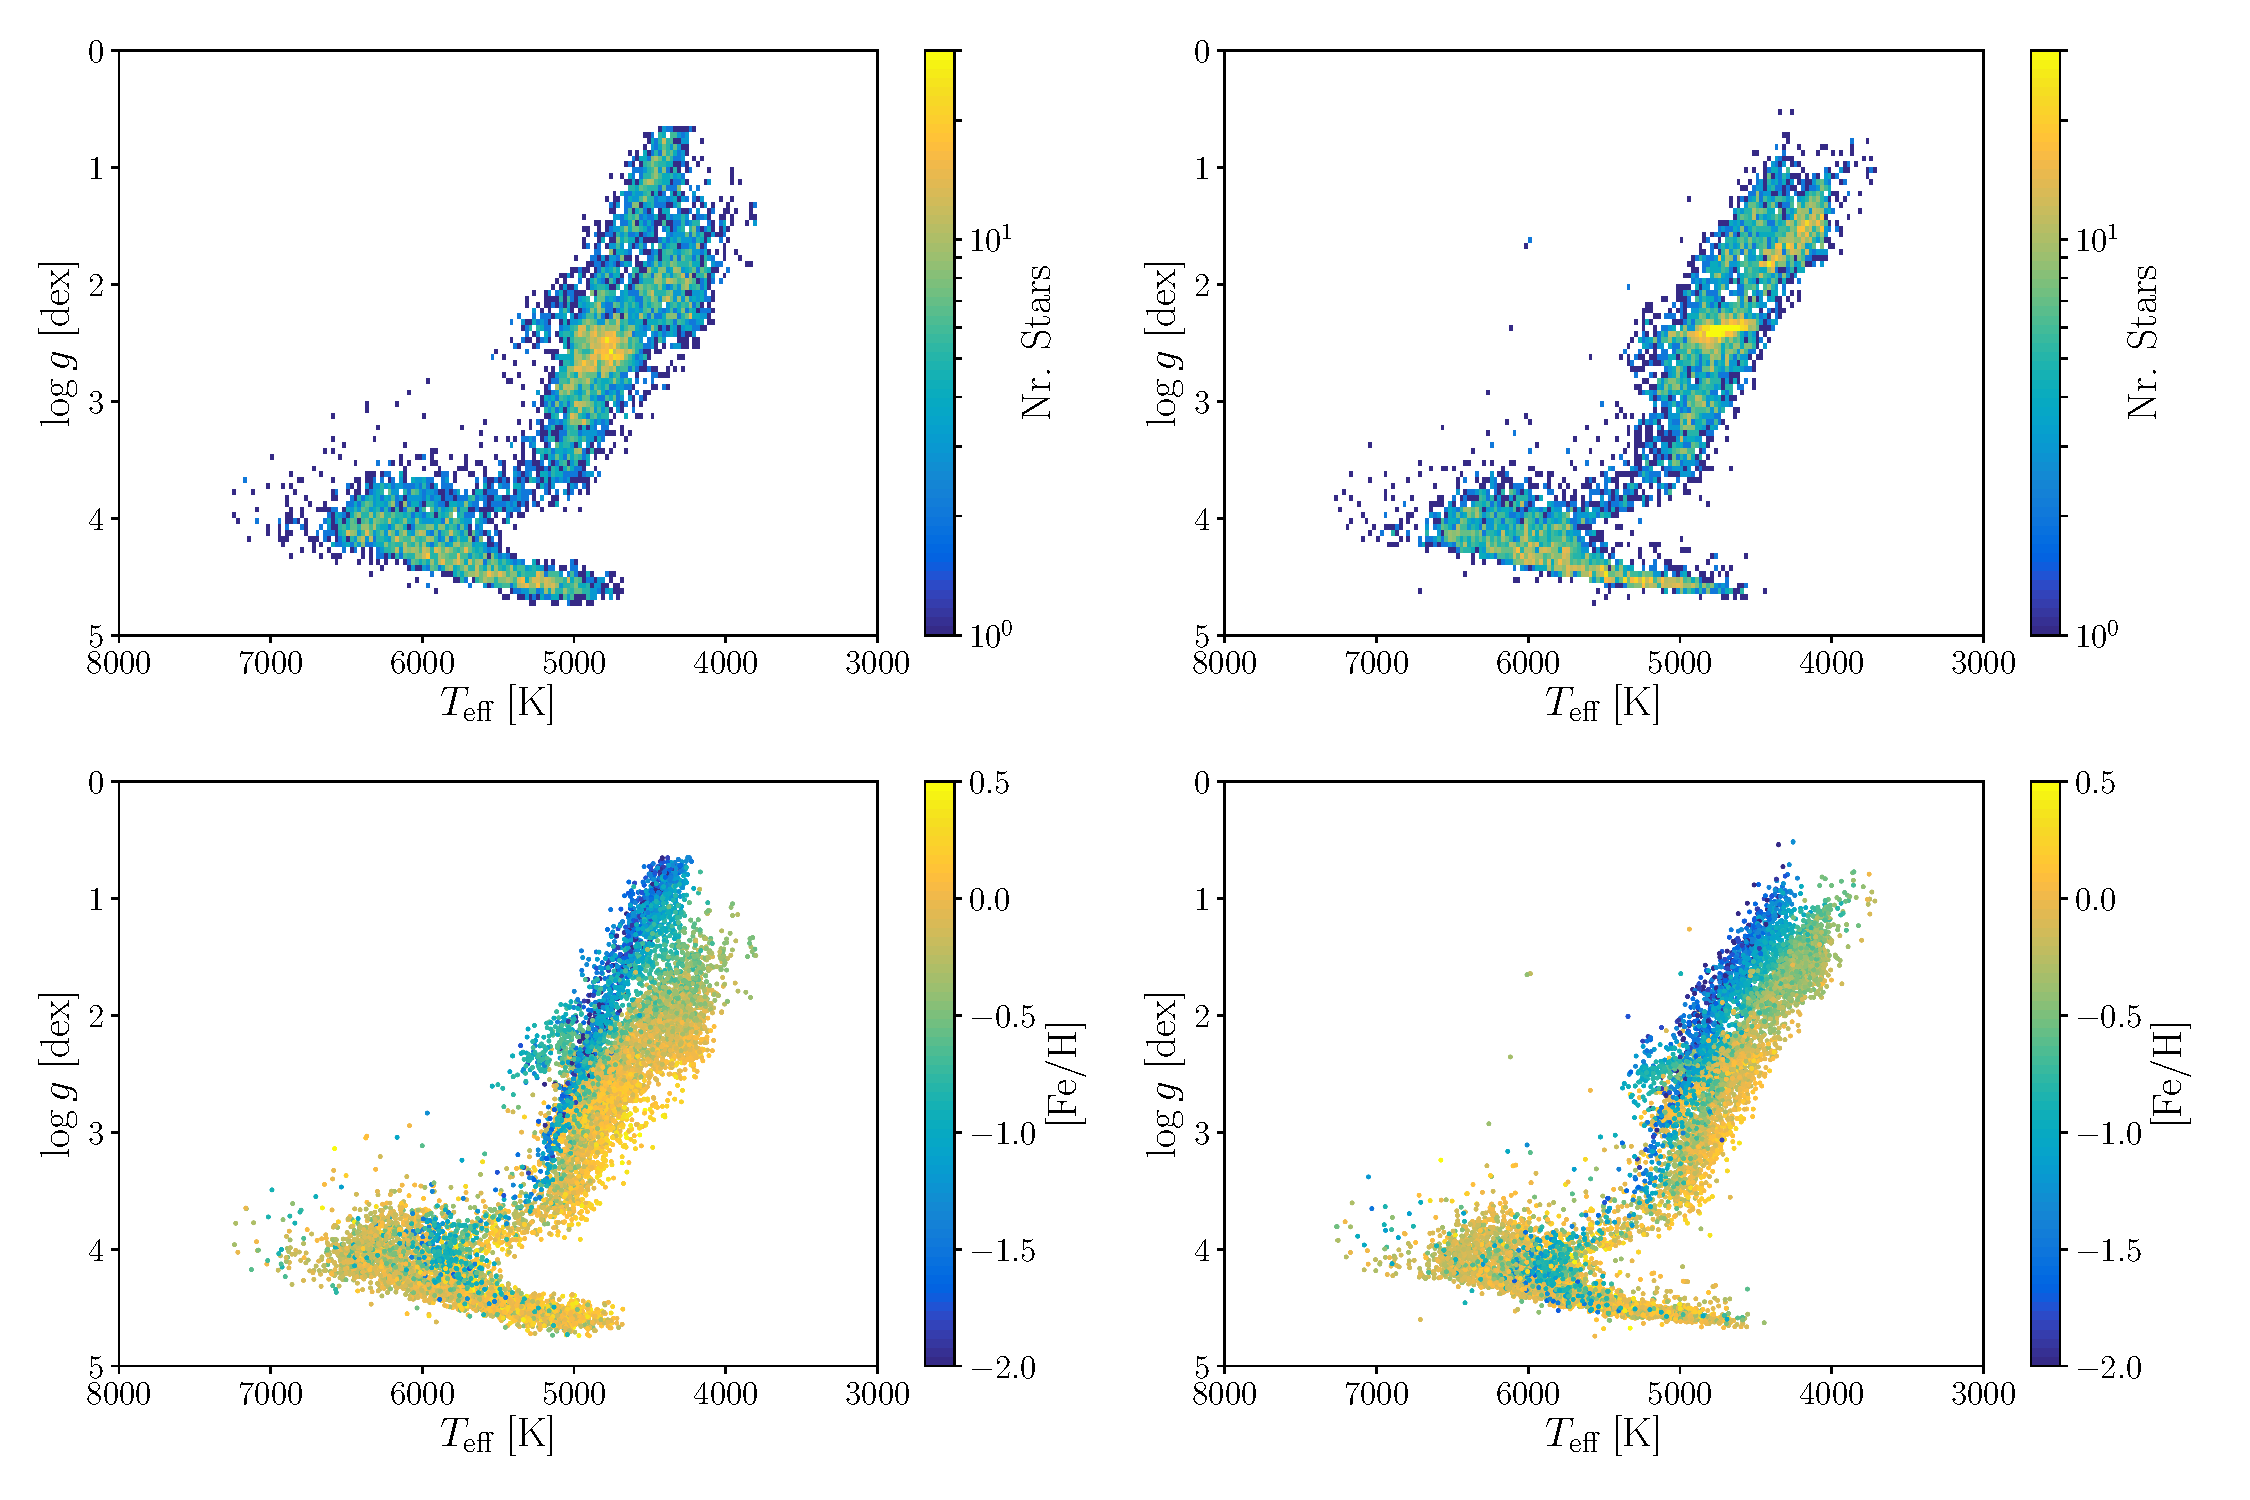
\includegraphics[width=\textwidth]{../../DR2_rerun/figures/dr2_rerun_kiel_comparison.pdf}
\caption{Comparison of kiel diagrams for GALAH DR2 training set (left panels: public DR2, right panels: current performance of the pipeline after the implementation of \textit{Gaia} DR2 information). Major improvements (including the red clump region) are described in the text.}
\label{fig:dr2_rerun_kiel}
\end{figure}

\subsection{Performances for 10000 randomly chosen spectra of the survey}

To achieve a more unbiased overview of the performance for the stars of the survey, we have randomly selected 10000 spectra and analysed them with the pipeline.

As can be seen in \autoref{fig:10000random}, this random sample includes more peculiar stars than the training set, most notably binaries (visible by the lower magnitude and $\log g$ in panels (a) and (b) due to the higher flux), stars with $\log g < 1$, hot and cool dwarfs ($T_text{eff} > 7000\,\mathrm{K}$ and $T_text{eff} < 4500\,\mathrm{K}$ respectively). With the exception of binaries, for which the stellar parameters are not trustworthy, the parameters have significantly improved at all parts of the parameter space. This includes the solved degeneracies in cool stars with many lines, which previously lead to a large scatter among the cool RGB stars and upturn (decreasing $\log g$ with decreasing $T_text{eff}$) for cool main sequence stars.

\begin{figure}[!ht]
\centering
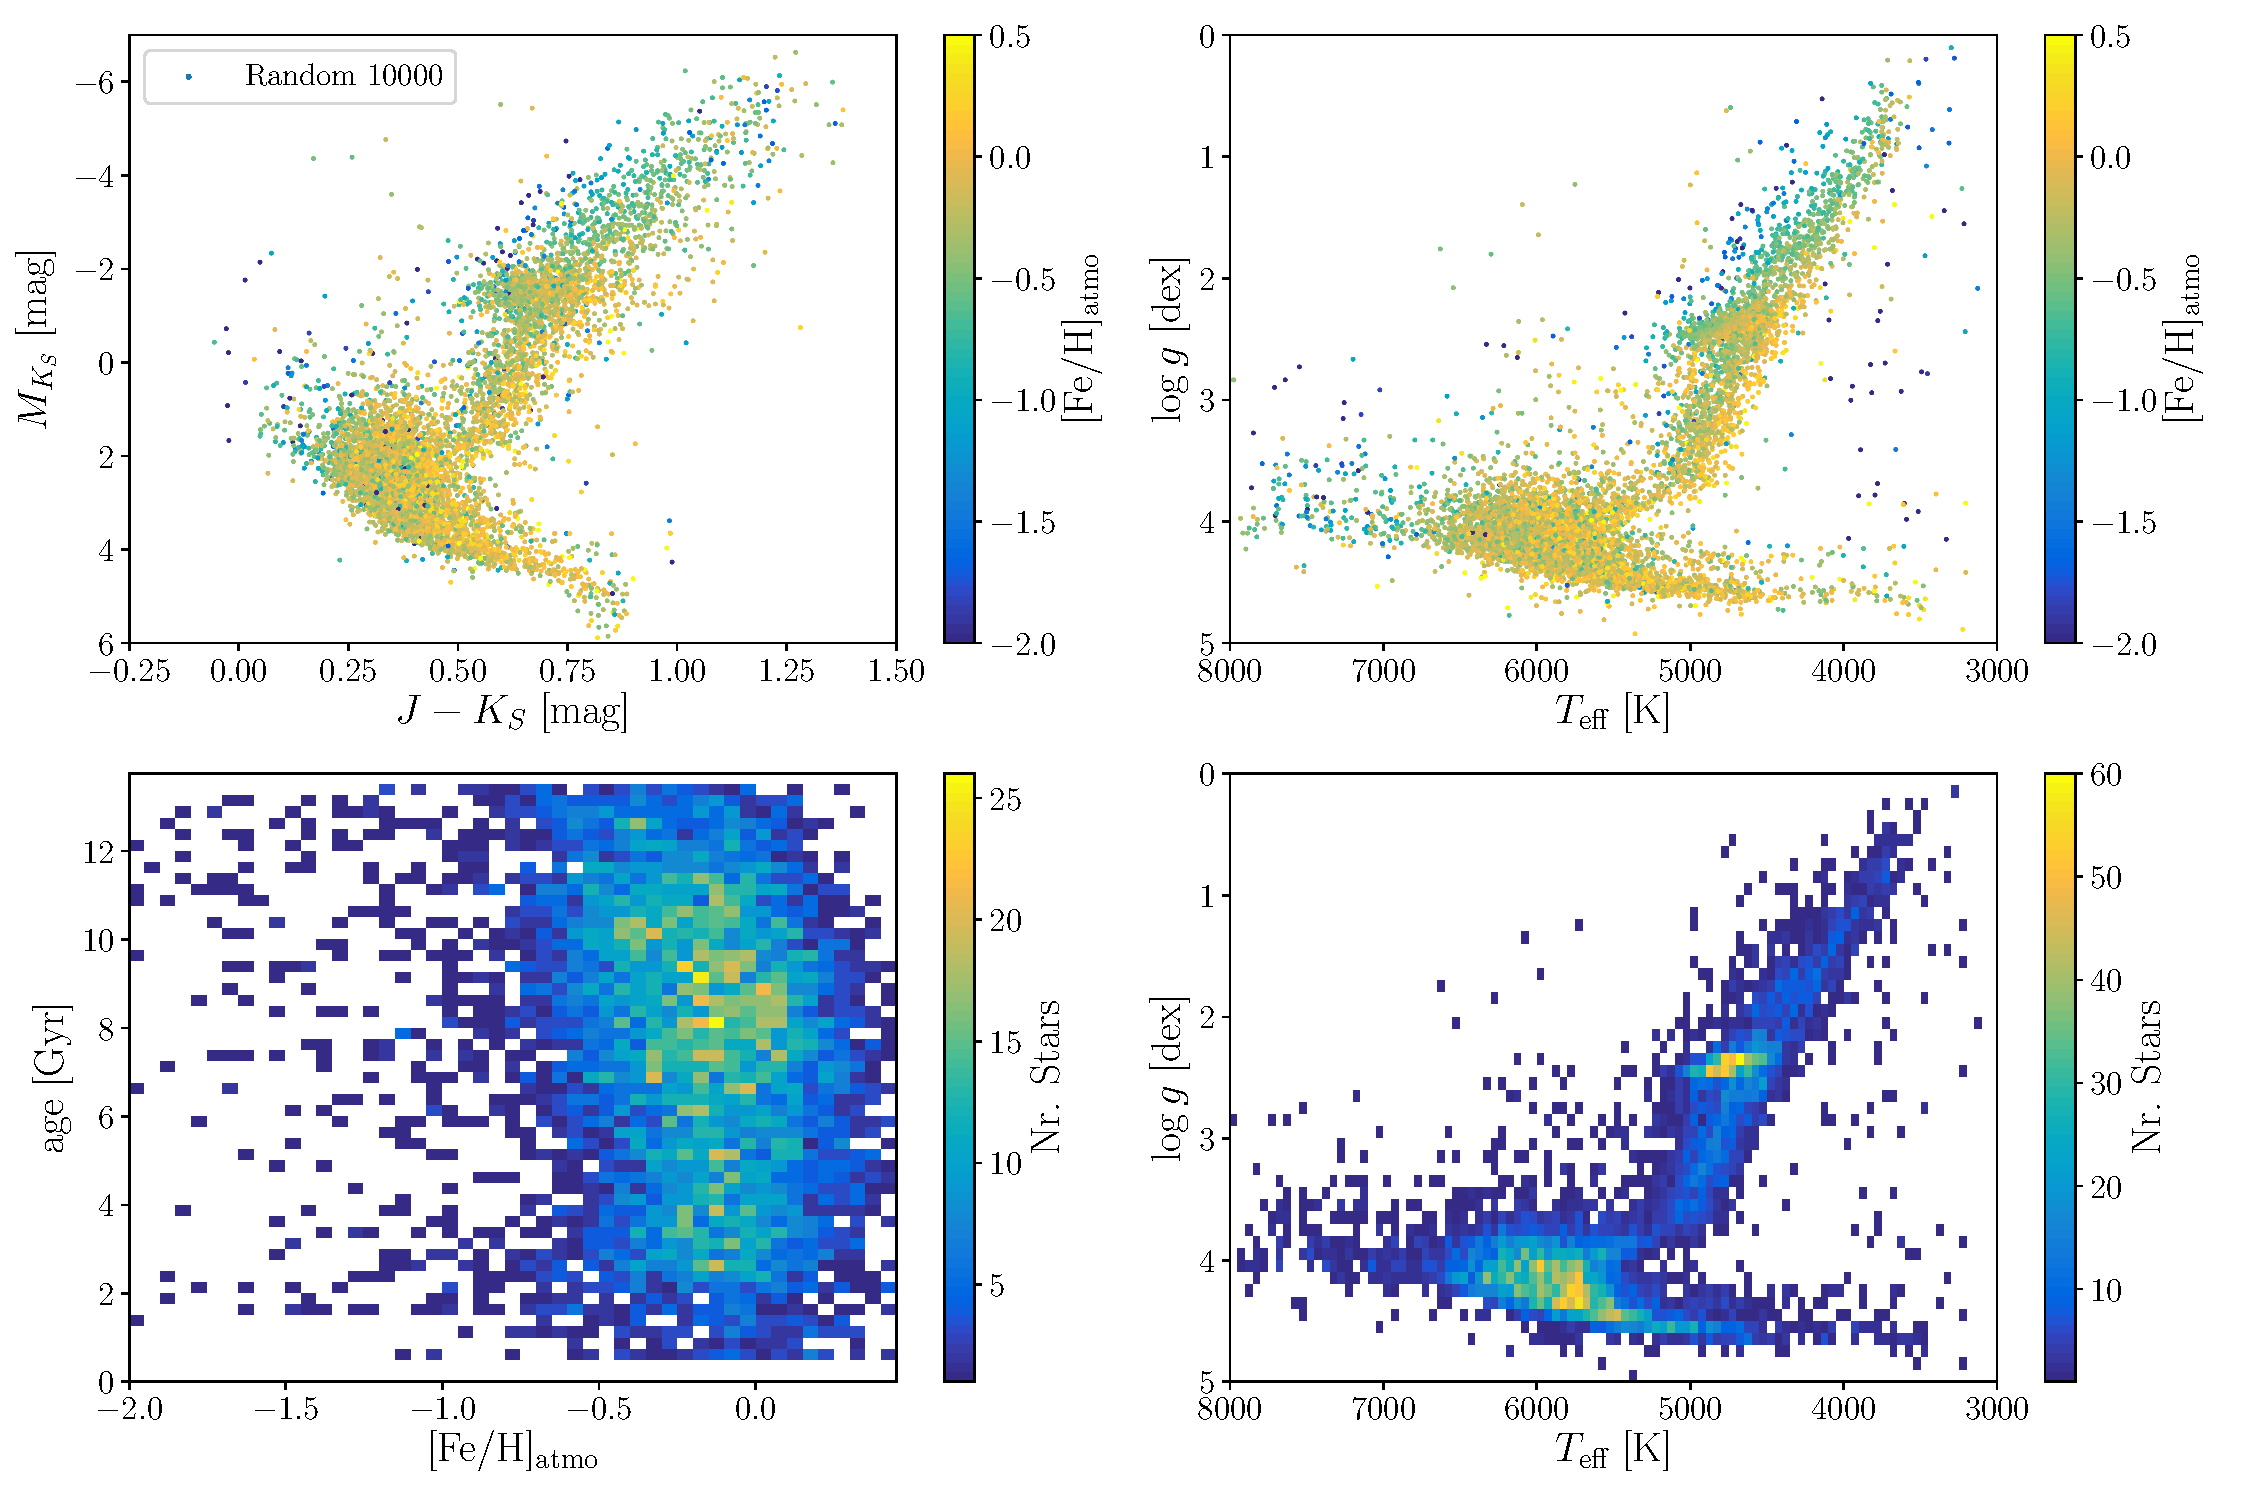
\includegraphics[width=\textwidth]{../../random10000/figures/random10000_cmdhrd.pdf}
\caption{Performance overview for 10000 randomly chosen spectra of the survey. (a) shows the color magnitude diagram with photometry from 2MASS (because 2MASS $K_S$ is used in the pipeline). (b) shows the Kiel diagram with parameters estimated from the pipeline, colored by the pseudo iron abundance of the model atmosphere. (c) show the pseudo iron abundance of the model atmosphere and the interim age estimation of the stars. The ages are not trustworthy, as they are a side product of the pipeline which concentrates on the mass estimation. (d) shows the density structure of the stars in a Kiel diagram with clear overdensities for red clumps and G dwarfs. More descriptions can be found in the text.}
\label{fig:10000random}
\end{figure}

In addition, we have been able to show that the pipeline can now also estimate stellar parameters of core-helium burning stars, including horizontal branch stars, which have not been included in the GALAH DR2 training set and are not significantly represented in the random sample. We have noted however, that for very distant stars (e.g. the bright stars in the LMC), the inferred distances by Bailer-Jones et al. (2018) are too low and hence lead to an overestimated $\log g$.

\newpage

\section{Future Tasks}

\subsection{Element abundances and their zeropoints}

The improvements in the SME implementations have decreased many offsets for the abundances estimated from spectra of the sky and Arcturus. However we still see differences for several elements both with respect to the literature (e.g. K) and between dwarf and giants (e.g. V). More work is needed to scrutinise the line selection and abundance zeropoints. The line-by-line analysis of element abundances has also been shown to been important for several elements (e.g. Al, Ca, and Ba) and has to be done to improve the accuracy and precision of abundance measurements.

\begin{figure}[!ht]
\centering
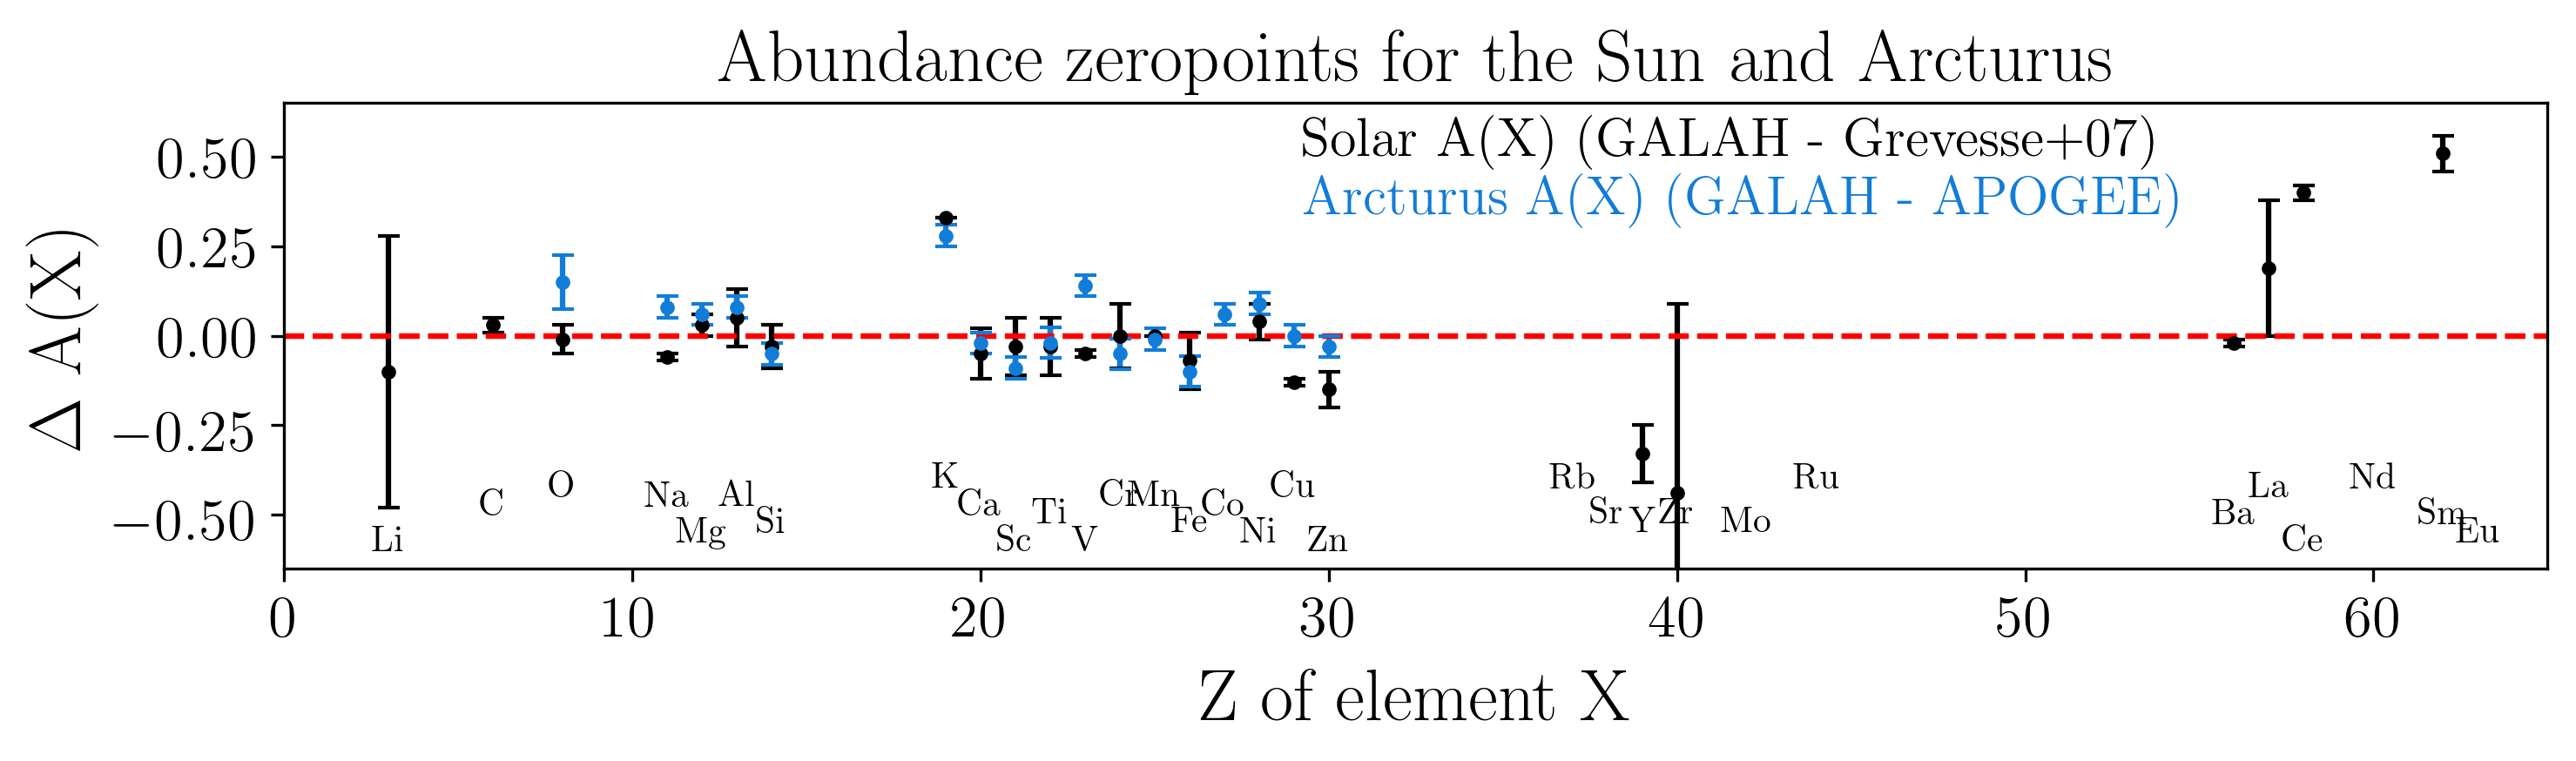
\includegraphics[width=\textwidth]{../../abundance_zeropoints/figures/abundance_zeropoints.png}
\caption{Abundance offsets between GALAH pipeline for a skyflat (150405000901378) and Arcturus (150210005801171).}
\label{fig:abundance_zeropoints}
\end{figure}

\subsection{Identification of binaries from photometry and spectroscopy}

Because we are now strongly connecting $\log g$ with the absolute magnitude, we will be strongly affected by spatially unresolved binaries, increasing the total flux and cause the estimated magnitude and $\log $ to be below the main sequence.

We hence need to implement more algorithms to identify binary stars from photometry, in addition to the spectroscopic identification.

\subsection{Reduction issues with the infrared arm}

Thanks to the effort of Janez and WG3, the IRAF reduction DR5.3 has improved the reduction of the spectra in many wavelength regions and we fully understand that not all changes can lead only to an improvement of the reduction.

Striving for even better analysis results, we would however like to ask for an improvement of the reduction and telluric correction for the infrared arm. We have seen the overcorrection of telluric lines among a significant percentage of stars leading to wrong normalisations and abundance analyses for all elements with lines in this arm.

%\section{Additional information: Dynamics}
%
%Sven Buder has calculated velocities and actions for all observed GALAH stars based on the \textit{Gaia} DR2 5D information and the radial velocities from WG3 (GUESS).
%
%The \href{https://github.com/svenbuder/GALAH_DR3/blob/master/dynamics/calculate_orbits.ipynb}{python script} is added added to the github repository and based on the following definitions:
%\begin{itemize}
%\item Uses Galpy 1.4  and its MWPotential2014
%\item Position of the sun: $R_{GC,\odot} = 8.2\,\mathrm{kpc}$, $z_{GC,\odot} = 25\,\mathrm{pc}$ (Bland-Hawthorn \& Gerhard 2016)
%\item $V_{LSR} = (-11, 10, 7.25)\,\mathrm{km/s}$ (Schoenrich+2012)
%\item Errors are MC sampled with 10000 draws, distance is sampled with 2-sided Gaussian sampling the distance estimates from Bailer-Jones+2018
%\item Calculated parameters: $X / Y / Z$, $U / V / W$, $R / \phi / z$, $J_R / L_Z / J_Z$, $e / z_\text{max} / R_\text{peri} / R_\text{ap}$ with means and standard deviations from MC sampling
%\item Use the estimated values $e / z_\text{max} / R_\text{peri} / R_\text{ap}$ with caution! More testing and confirmation is needed!
%\end{itemize}
%
%\begin{figure}[!ht]
%\centering
%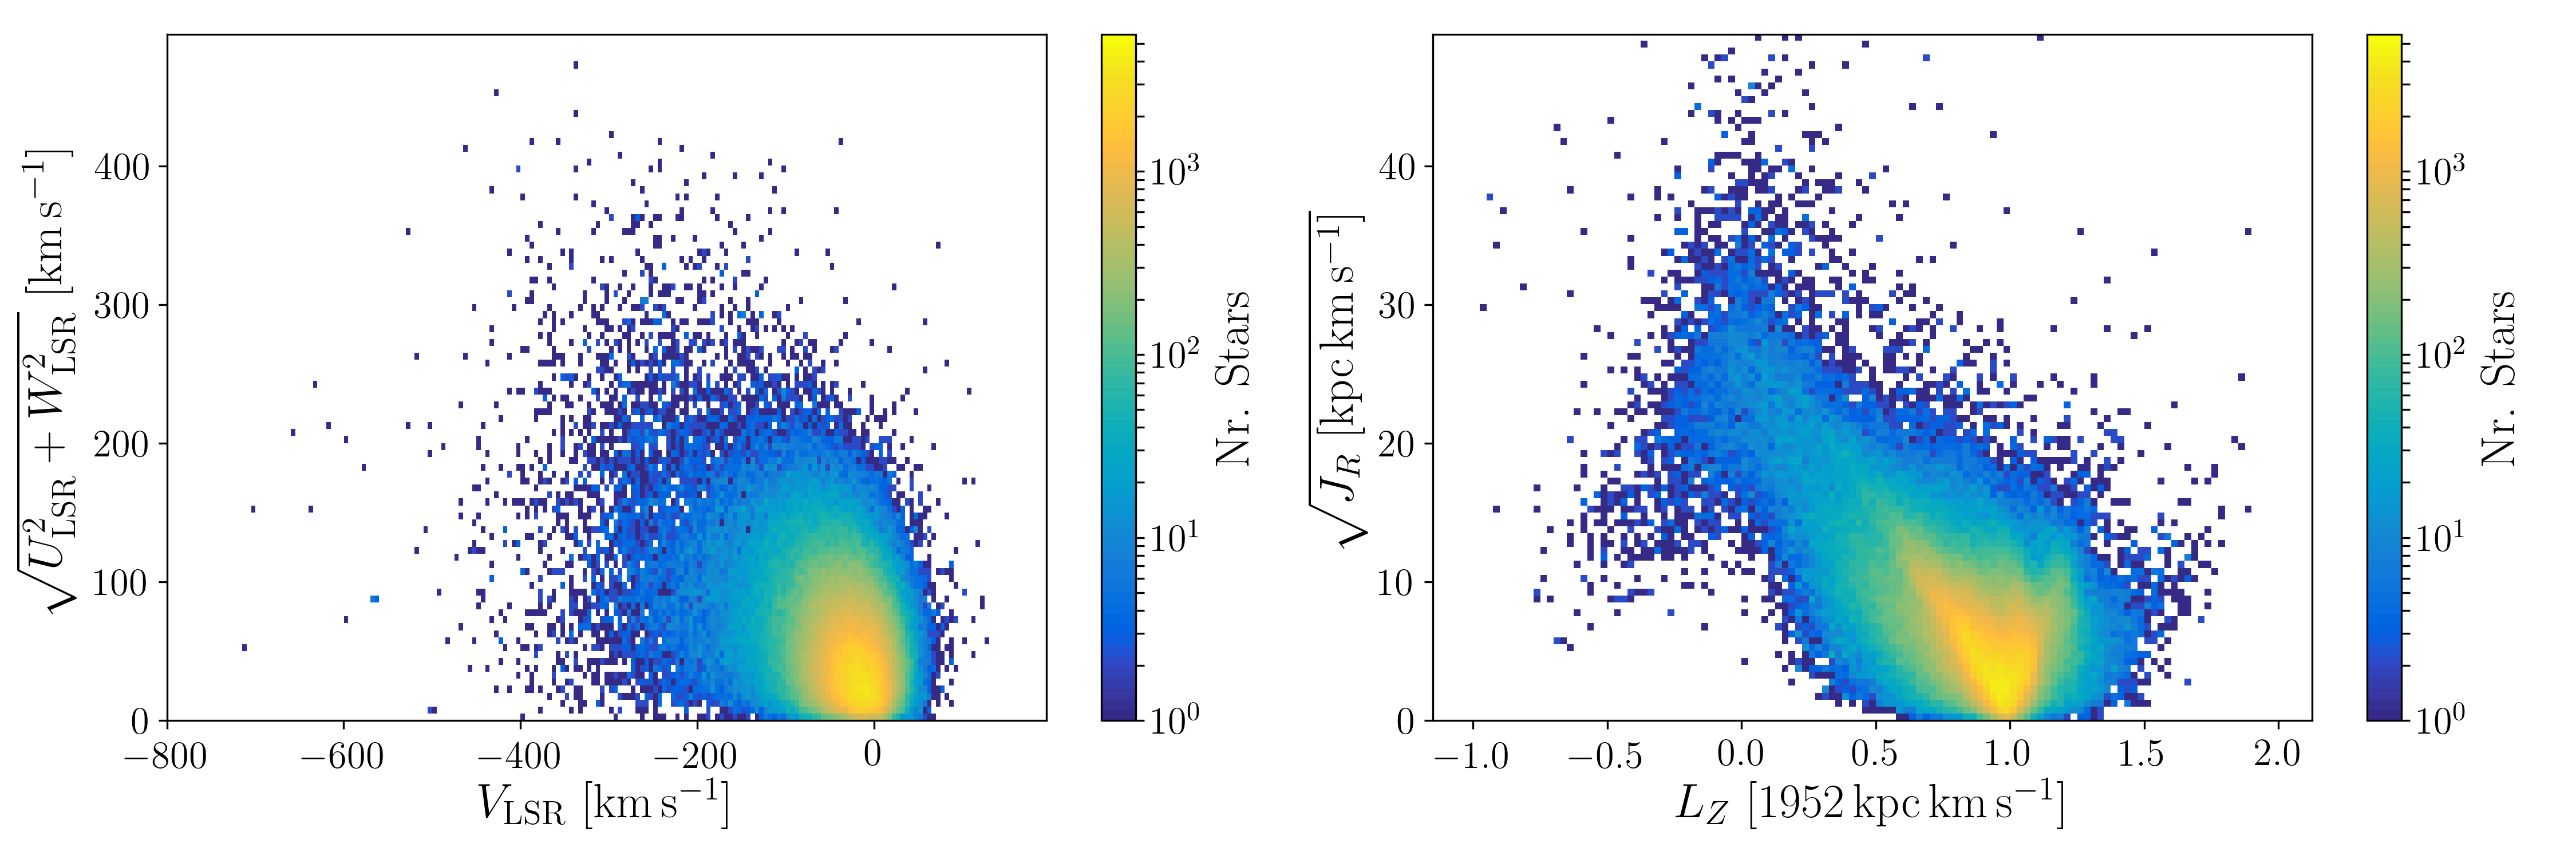
\includegraphics[width=\textwidth]{../../dynamics/figures/action_overview_clean_all.png}
%\caption{Overview of dynamics of stars observed by GALAH.}
%\label{fig:dynamics_overview}
%\end{figure}
%
%\begin{figure}[!ht]
%\centering
%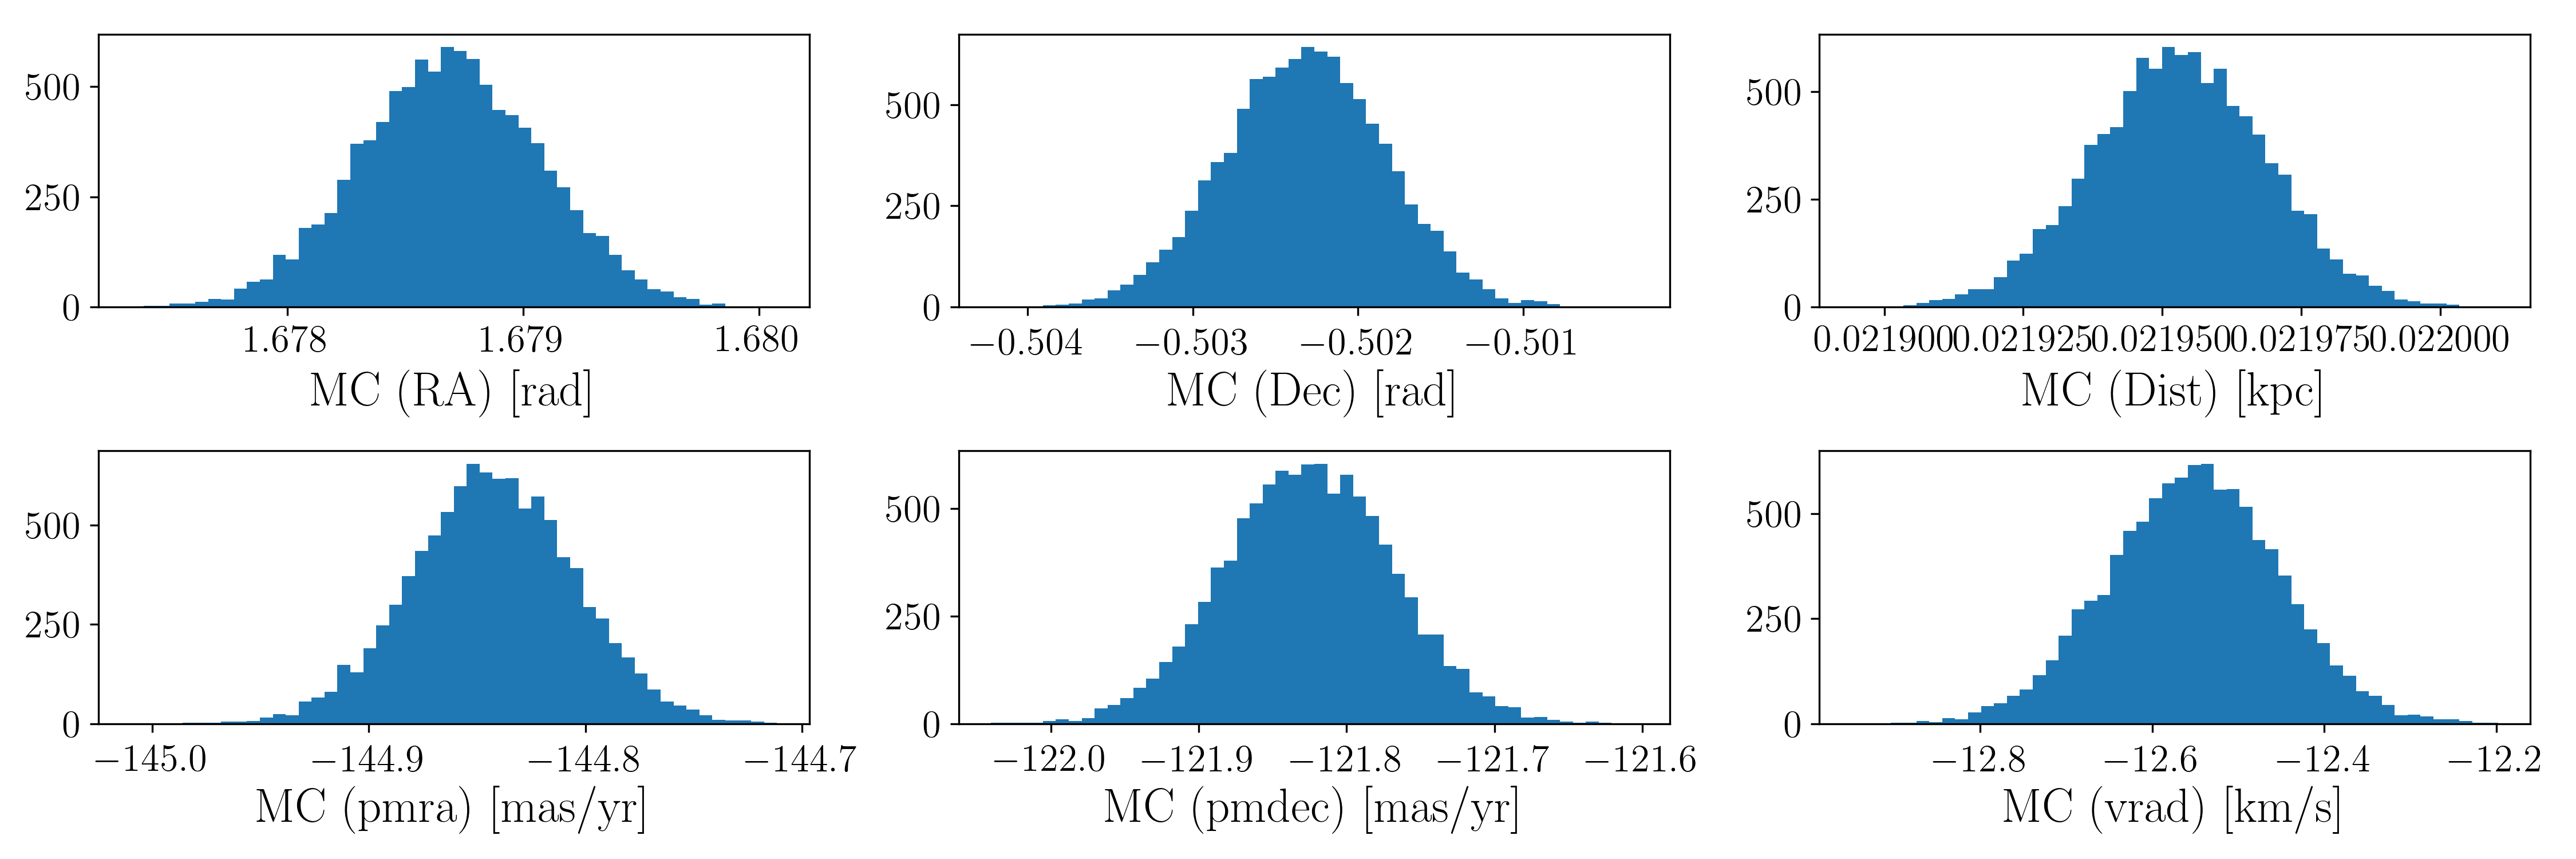
\includegraphics[width=\textwidth]{../../dynamics/figures/MC_input.png}
%\caption{Diagnostic plots of dynamic output from a subset of the GALAH sample.}
%\label{fig:dynamics_output}
%\end{figure}
%
%\begin{figure}[!ht]
%\centering
%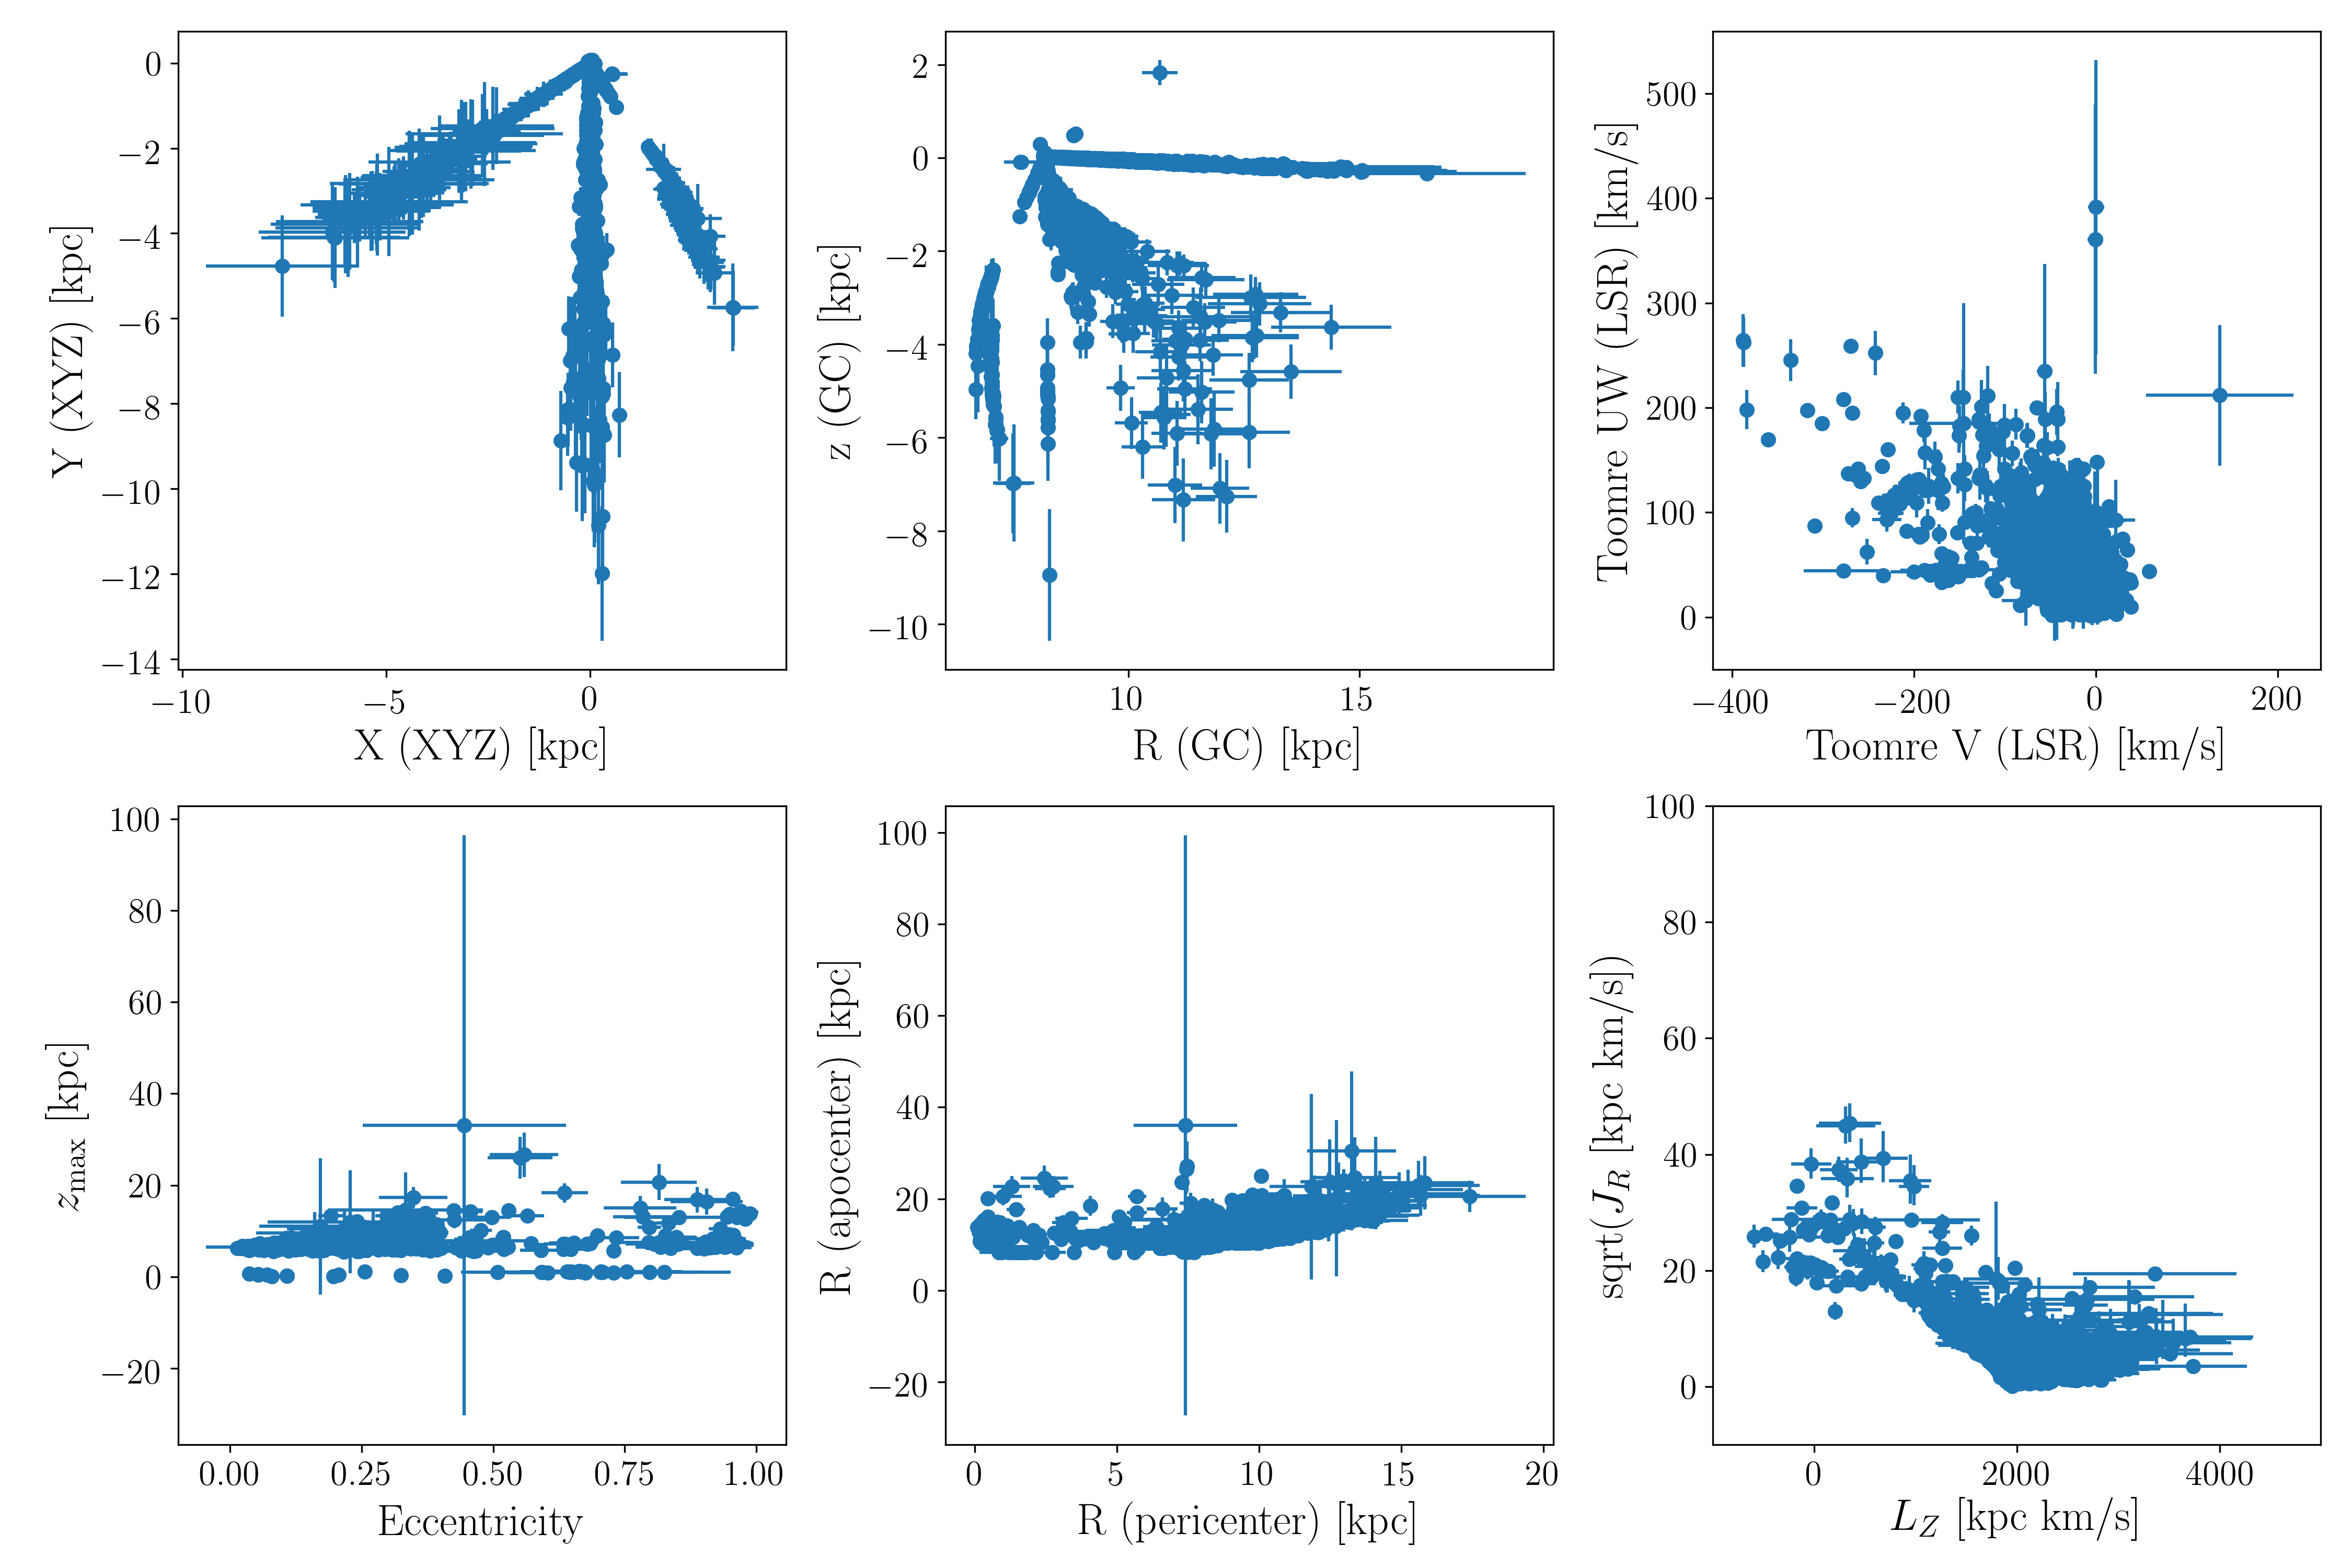
\includegraphics[width=\textwidth]{../../dynamics/figures/MC_output.png}
%\caption{Diagnostic plots of dynamic output from a subset of the GALAH sample.}
%\label{fig:dynamics_input}
%\end{figure}
%
\end{document}